% Nature Communications — Article
%DIF LATEXDIFF DIFFERENCE FILE
%DIF DEL submission_revision_v1/ncomms_main_post_T5.tex   Sun May 10 22:14:27 2026
%DIF ADD article/ncomms_main.tex                          Tue May 12 15:27:06 2026
% "Same Prompt, Different Answer: Hidden Non-Determinism in LLM APIs
%  Undermines Scientific Reproducibility"
%
% Formatted using the official Springer Nature sn-jnl template
% with sn-nature style for Nature Portfolio journals.

\documentclass[sn-nature]{sn-jnl}

%%%% Packages
\usepackage{graphicx}
\usepackage{multirow}
\usepackage{amsmath,amssymb,amsfonts}
\usepackage{amsthm}
\usepackage{xcolor}
\usepackage{textcomp}
\usepackage{manyfoot}
\usepackage{booktabs}
\usepackage[title]{appendix}
\usepackage{colortbl}
\usepackage{lineno}

%DIF 23a23-25
% ORCID inline link helper (orcidlink package not available in some TeX distributions) %DIF > 
\providecommand{\orcidlink}[1]{\href{https://orcid.org/#1}{\textsuperscript{\textsf{\scriptsize ORCID}}}} %DIF > 
 %DIF > 
%DIF -------
\raggedbottom
\unnumbered% Nature Communications uses unnumbered section heads
%DIF PREAMBLE EXTENSION ADDED BY LATEXDIFF
%DIF UNDERLINE PREAMBLE %DIF PREAMBLE
\RequirePackage[normalem]{ulem} %DIF PREAMBLE
\RequirePackage{color}\definecolor{RED}{rgb}{1,0,0}\definecolor{BLUE}{rgb}{0,0,1} %DIF PREAMBLE
\providecommand{\DIFadd}[1]{{\protect\color{blue}\uwave{#1}}} %DIF PREAMBLE
\providecommand{\DIFdel}[1]{{\protect\color{red}\sout{#1}}} %DIF PREAMBLE
%DIF SAFE PREAMBLE %DIF PREAMBLE
\providecommand{\DIFaddbegin}{} %DIF PREAMBLE
\providecommand{\DIFaddend}{} %DIF PREAMBLE
\providecommand{\DIFdelbegin}{} %DIF PREAMBLE
\providecommand{\DIFdelend}{} %DIF PREAMBLE
\providecommand{\DIFmodbegin}{} %DIF PREAMBLE
\providecommand{\DIFmodend}{} %DIF PREAMBLE
%DIF FLOATSAFE PREAMBLE %DIF PREAMBLE
\providecommand{\DIFaddFL}[1]{\DIFadd{#1}} %DIF PREAMBLE
\providecommand{\DIFdelFL}[1]{\DIFdel{#1}} %DIF PREAMBLE
\providecommand{\DIFaddbeginFL}{} %DIF PREAMBLE
\providecommand{\DIFaddendFL}{} %DIF PREAMBLE
\providecommand{\DIFdelbeginFL}{} %DIF PREAMBLE
\providecommand{\DIFdelendFL}{} %DIF PREAMBLE
\providecommand{\DIFscaledelfig}{0.5}
%DIF HIGHLIGHTGRAPHICS PREAMBLE %DIF PREAMBLE
\RequirePackage{settobox} %DIF PREAMBLE
\RequirePackage{letltxmacro} %DIF PREAMBLE
\newsavebox{\DIFdelgraphicsbox} %DIF PREAMBLE
\newlength{\DIFdelgraphicswidth} %DIF PREAMBLE
\newlength{\DIFdelgraphicsheight} %DIF PREAMBLE
% store original definition of \includegraphics %DIF PREAMBLE
\LetLtxMacro{\DIFOincludegraphics}{\includegraphics} %DIF PREAMBLE
\providecommand{\DIFaddincludegraphics}[2][]{{\color{blue}\fbox{\DIFOincludegraphics[#1]{#2}}}} %DIF PREAMBLE
\providecommand{\DIFdelincludegraphics}[2][]{% %DIF PREAMBLE
\sbox{\DIFdelgraphicsbox}{\DIFOincludegraphics[#1]{#2}}% %DIF PREAMBLE
\settoboxwidth{\DIFdelgraphicswidth}{\DIFdelgraphicsbox} %DIF PREAMBLE
\settoboxtotalheight{\DIFdelgraphicsheight}{\DIFdelgraphicsbox} %DIF PREAMBLE
\scalebox{\DIFscaledelfig}{% %DIF PREAMBLE
\parbox[b]{\DIFdelgraphicswidth}{\usebox{\DIFdelgraphicsbox}\\[-\baselineskip] \rule{\DIFdelgraphicswidth}{0em}}\llap{\resizebox{\DIFdelgraphicswidth}{\DIFdelgraphicsheight}{% %DIF PREAMBLE
\setlength{\unitlength}{\DIFdelgraphicswidth}% %DIF PREAMBLE
\begin{picture}(1,1)% %DIF PREAMBLE
\thicklines\linethickness{2pt} %DIF PREAMBLE
{\color[rgb]{1,0,0}\put(0,0){\framebox(1,1){}}}% %DIF PREAMBLE
{\color[rgb]{1,0,0}\put(0,0){\line( 1,1){1}}}% %DIF PREAMBLE
{\color[rgb]{1,0,0}\put(0,1){\line(1,-1){1}}}% %DIF PREAMBLE
\end{picture}% %DIF PREAMBLE
}\hspace*{3pt}}} %DIF PREAMBLE
} %DIF PREAMBLE
\LetLtxMacro{\DIFOaddbegin}{\DIFaddbegin} %DIF PREAMBLE
\LetLtxMacro{\DIFOaddend}{\DIFaddend} %DIF PREAMBLE
\LetLtxMacro{\DIFOdelbegin}{\DIFdelbegin} %DIF PREAMBLE
\LetLtxMacro{\DIFOdelend}{\DIFdelend} %DIF PREAMBLE
\DeclareRobustCommand{\DIFaddbegin}{\DIFOaddbegin \let\includegraphics\DIFaddincludegraphics} %DIF PREAMBLE
\DeclareRobustCommand{\DIFaddend}{\DIFOaddend \let\includegraphics\DIFOincludegraphics} %DIF PREAMBLE
\DeclareRobustCommand{\DIFdelbegin}{\DIFOdelbegin \let\includegraphics\DIFdelincludegraphics} %DIF PREAMBLE
\DeclareRobustCommand{\DIFdelend}{\DIFOaddend \let\includegraphics\DIFOincludegraphics} %DIF PREAMBLE
\LetLtxMacro{\DIFOaddbeginFL}{\DIFaddbeginFL} %DIF PREAMBLE
\LetLtxMacro{\DIFOaddendFL}{\DIFaddendFL} %DIF PREAMBLE
\LetLtxMacro{\DIFOdelbeginFL}{\DIFdelbeginFL} %DIF PREAMBLE
\LetLtxMacro{\DIFOdelendFL}{\DIFdelendFL} %DIF PREAMBLE
\DeclareRobustCommand{\DIFaddbeginFL}{\DIFOaddbeginFL \let\includegraphics\DIFaddincludegraphics} %DIF PREAMBLE
\DeclareRobustCommand{\DIFaddendFL}{\DIFOaddendFL \let\includegraphics\DIFOincludegraphics} %DIF PREAMBLE
\DeclareRobustCommand{\DIFdelbeginFL}{\DIFOdelbeginFL \let\includegraphics\DIFdelincludegraphics} %DIF PREAMBLE
\DeclareRobustCommand{\DIFdelendFL}{\DIFOaddendFL \let\includegraphics\DIFOincludegraphics} %DIF PREAMBLE
%DIF AMSMATHULEM PREAMBLE %DIF PREAMBLE
\makeatletter %DIF PREAMBLE
\let\sout@orig\sout %DIF PREAMBLE
\renewcommand{\sout}[1]{\ifmmode\text{\sout@orig{\ensuremath{#1}}}\else\sout@orig{#1}\fi} %DIF PREAMBLE
\makeatother %DIF PREAMBLE
%DIF COLORLISTINGS PREAMBLE %DIF PREAMBLE
\RequirePackage{listings} %DIF PREAMBLE
\RequirePackage{color} %DIF PREAMBLE
\lstdefinelanguage{DIFcode}{ %DIF PREAMBLE
%DIF DIFCODE_UNDERLINE %DIF PREAMBLE
  moredelim=[il][\color{red}\sout]{\%DIF\ <\ }, %DIF PREAMBLE
  moredelim=[il][\color{blue}\uwave]{\%DIF\ >\ } %DIF PREAMBLE
} %DIF PREAMBLE
\lstdefinestyle{DIFverbatimstyle}{ %DIF PREAMBLE
	language=DIFcode, %DIF PREAMBLE
	basicstyle=\ttfamily, %DIF PREAMBLE
	columns=fullflexible, %DIF PREAMBLE
	keepspaces=true %DIF PREAMBLE
} %DIF PREAMBLE
\lstnewenvironment{DIFverbatim}[1][]{\lstset{style=DIFverbatimstyle}}{} %DIF PREAMBLE
\lstnewenvironment{DIFverbatim*}[1][]{\lstset{style=DIFverbatimstyle,showspaces=true}}{} %DIF PREAMBLE
\lstset{extendedchars=\true,inputencoding=utf8}

%DIF END PREAMBLE EXTENSION ADDED BY LATEXDIFF

\begin{document}

\title[Same Prompt, Different Answer]{Same Prompt, Different Answer: Hidden Non-Determinism in LLM APIs Undermines Scientific Reproducibility}

%%=============================================================%%
%% Authors
%%=============================================================%%

\DIFdelbegin %DIFDELCMD < \author*[1]{\fnm{Lucas} \sur{Rover}}%%%
\DIFdelend \DIFaddbegin \author*[1]{\fnm{Lucas} \sur{Rover}~\orcidlink{0000-0001-6641-9224}}\DIFaddend \email{lucasrover@alunos.utfpr.edu.br}
\equalcont{Corresponding author.}
%DIF < % ORCID: 0000-0001-6641-9224 (entered via Editorial Manager at submission)

\author[1]{\fnm{Hugo Valadares} \sur{Siqueira}\DIFaddbegin \DIFadd{~\orcidlink{0000-0002-1278-4602}}\DIFaddend }

\author[2]{\fnm{Eduardo Tadeu} \sur{Bacalhau}\DIFaddbegin \DIFadd{~\orcidlink{0000-0002-3936-0375}}\DIFaddend }

\author[3]{\fnm{Anibal Tavares} \spfx{de} \sur{Azevedo}\DIFaddbegin \DIFadd{~\orcidlink{0000-0003-1678-7795}}\DIFaddend }

\author[1]{\fnm{Yara} \spfx{de Souza} \sur{Tadano}\DIFaddbegin \DIFadd{~\orcidlink{0000-0002-3975-3419}}\DIFaddend }

\DIFdelbegin %DIFDELCMD < \affil*[1]{\orgdiv{Graduate Program in Mechanical Engineering},
%DIFDELCMD < \orgname{Federal University of Technology --- Paran\'a (UTFPR)},
%DIFDELCMD < \orgaddress{\city{Ponta Grossa}, \state{Paran\'a}, \country{Brazil}}}
%DIFDELCMD < %%%
\DIFdelend \DIFaddbegin \affil*[1]{\orgname{Federal University of Technology --- Paran\'a (UTFPR)},
\orgaddress{\country{Brazil}}}
\DIFaddend 

\DIFdelbegin \DIFdel{\affil[2]{\orgdiv{Research Group of Technology Applied to Optimization (GTAO)},
\orgname{Federal University of Paran\'a (UFPR)},
\orgaddress{\city{Curitiba}, \state{Paran\'a}, \country{Brazil}}}
}\DIFdelend \DIFaddbegin \DIFadd{\affil[2]{\orgname{Federal University of Paran\'a (UFPR)},
\orgaddress{\country{Brazil}}}
}\DIFaddend 

\DIFdelbegin \DIFdel{\affil[3]{\orgdiv{School of Applied Sciences (FCA)},
\orgname{University of Campinas (Unicamp)},
\orgaddress{\city{Limeira}, \state{S\~ao Paulo}, \country{Brazil}}}
}\DIFdelend \DIFaddbegin \DIFadd{\affil[3]{\orgname{University of Campinas (Unicamp)},
\orgaddress{\country{Brazil}}}
}\DIFaddend 

%%=============================================================%%
%% Abstract (~150 words, unreferenced)
%%=============================================================%%

\DIFdelbegin %DIFDELCMD < \abstract{Thousands of published studies across medicine, climate science, and engineering report results generated by large language model APIs under settings documented as deterministic, yet we show that this guarantee does not hold in practice.
%DIFDELCMD < In 4,104 controlled experiments across nine \emph{deployment stacks}---tuples of (model weights, provider, serving infrastructure, API layer)---spanning eight models and five API providers, API-served stacks reproduce their own outputs only 22\% of the time under temperature-zero greedy decoding with fixed seeds, while locally deployed stacks achieve 96\%---a gap exceeding four-fold.
%DIFDELCMD < This variation is invisible to researchers: outputs remain semantically equivalent (BERTScore F1~$>$~0.97) while differing textually, meaning that non-identical results escape detection without systematic comparison.
%DIFDELCMD < The problem amplifies in multi-turn and retrieval-augmented generation workflows, where one stack produces zero exact matches across 50 runs.
%DIFDELCMD < A quasi-isolation experiment in which the same LLaMA~3 8B weights are served by two different stacks attributes the cause to production infrastructure complexity rather than cloud deployment itself, showing the problem is solvable.
%DIFDELCMD < We provide a lightweight provenance protocol ($<$1\% overhead) grounded in W3C PROV that makes this hidden variation detectable and auditable, offering practical infrastructure for reproducible LLM-based research.}
%DIFDELCMD < %%%
\DIFdelend \DIFaddbegin \abstract{Large language model APIs serve research in medicine, climate science, and engineering under settings documented as deterministic. We show this guarantee fails in practice. Across 7{,}004 experiments on nine \emph{deployment stacks} (weights, provider, infrastructure, API) and six task families (extraction, summarisation, multi-turn refinement, RAG, code, math), API-served stacks reproduce their own outputs as little as 1\% under temperature-zero greedy decoding with fixed seeds, while local-stack averages reach 93--98\%. The variation is invisible: outputs appear semantically equivalent (BERTScore F1~$>$~0.97) but diverge textually, yet two blinded LLM judges (Claude Opus 4.7, gpt-4o) classify the majority (73--90\%) as truly contradictory. The gap widens in high-stakes regimes (multi-turn, RAG, code, math). A quasi-isolation experiment with identical LLaMA~3~8B weights on two stacks implicates production infrastructure rather than cloud deployment. We release a W3C PROV-based provenance protocol ($<$1\% overhead) making this hidden variation auditable.}
\DIFaddend 

\keywords{Reproducibility, Large language models, Non-determinism, Provenance, API inference}

\maketitle

\linenumbers

%%=============================================================%%
%% MAIN TEXT --- Opening paragraphs (no heading)
%%=============================================================%%

Large language models (LLMs) are rapidly becoming standard research instruments.
They encode clinical knowledge\cite{singhal2023large}, assist diagnostic workflows\cite{thirunavukarasu2023large}, accelerate literature review and data extraction\cite{birhane2023science}, and are increasingly integrated into peer review at scale\cite{thakkar2026llm}.
A growing body of work deploys LLMs as evaluators of human communication\cite{kumar2026reliable}, as psychometric assessment tools\cite{serapiogarcía2025psychometric}, and as components of multi-agent scientific pipelines\cite{xin2025agentic}.
When researchers use API-based models, they trust that identical configurations will yield identical outputs.
API documentation reinforces this trust by offering a temperature parameter set to zero for ``deterministic'' behavio\DIFaddbegin \DIFadd{u}\DIFaddend r , a setting that should collapse the output probability distribution to a single token at each step.
Our experiments show that this guarantee does not hold.

The broader reproducibility crisis in science is well documented: over 70\% of researchers have failed to reproduce another scientist's experiment\cite{baker2016reproducibility}, and the problem is acute in AI, where only 6\% of papers provide sufficient information for reproduction\cite{gundersen2018state}.
The field faces its own ``reproducibility crisis''\cite{hutson2018artificial}, with growing concerns that AI may worsen the problem across disciplines\cite{ball2023ai}.
Data leakage alone has been documented across 17 machine learning subfields\cite{kapoor2023leakage}, and leading AI journals have begun adopting structured reproducibility mechanisms in response\cite{gundersen2024improving}.
Yet despite this attention to training-time reproducibility, the reproducibility of \emph{inference}, the actual deployment of models to generate outputs, remains largely unexamined.
This gap matters because inference is the stage at which LLMs interact with research data and produce the outputs that enter scientific records, policy documents, and clinical workflows.
Existing experiment-tracking tools such as MLflow\cite{zaharia2018accelerating} were designed for training pipelines and numerical metrics, not for inference-time text-generation provenance.

We conducted \DIFdelbegin \DIFdel{4,104 }\DIFdelend \DIFaddbegin \DIFadd{7}{\DIFadd{,}}\DIFadd{004 }\DIFaddend controlled experiments across \DIFdelbegin \DIFdel{eight models and }\DIFdelend \DIFaddbegin \DIFadd{nine deployment stacks, eight models (counting OpenAI's GPT-4 family---gpt-4-0613 from the original analysis plus the revision-batch gpt-4o-2024-11-20 snapshot---as a single model, and LLaMA~3 8B once despite being served on two stacks), }\DIFaddend five independent API providers\DIFdelbegin \DIFdel{and }\DIFdelend \DIFaddbegin \DIFadd{, and six task families: structured extraction, scientific summarisation, multi-turn refinement, retrieval-augmented generation, code generation (HumanEval), and mathematical reasoning (GSM8K). The original analysis contributed 4}{\DIFadd{,}}\DIFadd{104 of these and the major-revision additions contributed the remaining 2}{\DIFadd{,}}\DIFadd{900.
We }\DIFaddend found that even under temperature~$=$~0 with fixed random seeds, API-served models reproduce their own outputs only 22.1\% of the time \DIFdelbegin \DIFdel{, while locally }\DIFdelend \DIFaddbegin \DIFadd{on the original two tasks (averaged across GPT-4 and Claude Sonnet 4.5, the two API stacks with full Tasks~1--4 coverage). Locally }\DIFaddend deployed open-weight models achieve 95.6\% exact reproducibility \DIFdelbegin \DIFdel{, a gap exceeding four-fold (}\DIFdelend \DIFaddbegin \DIFadd{on the same tasks---a ratio of approximately $4\times$ in point estimates ($3.1\times$ under the balanced 10-abstract subsample, }\DIFaddend 95\% bootstrap CI\DIFdelbegin \DIFdel{for the ratio}\DIFdelend : 2.48--3.61$\times$\DIFdelbegin \DIFdel{)}\DIFdelend \DIFaddbegin \DIFadd{; Extended Data Table~4), with the revision experiments confirming the gap extends to code, math, and out-of-AI/ML domains}\DIFaddend .
This non-determinism is invisible to users: outputs are semantically equivalent (BERTScore F1~$>$~0.97) but textually different, meaning researchers cannot detect the variation by reading outputs.
The phenomenon is not confined to single queries.
As LLMs move into agentic pipelines that design experiments and generate hypotheses\cite{xin2025agentic}, this hidden variation compounds at every step.
Recent editorials have underscored the urgency of transparency in multi-agent AI systems\cite{editorial2026multiagent}, yet the baseline reproducibility of the individual API calls has never been systematically quantified.

A central conceptual point underlies our analysis: when a researcher queries an LLM through an API, the experimental object is not a model in the abstract sense but a \emph{deployment stack}, the tuple (model weights, provider, serving infrastructure, API layer).
The same weights served by two different stacks can yield two different reproducibility profiles, because each component of the tuple can independently introduce variation through tensor parallelism, mixed-precision accumulation, dynamic batching, or post-processing.
We therefore frame results per stack rather than per model: identifiers such as ``GPT-4'' refer throughout to the full deployment stack served by the provider at the time of measurement, not to a model abstraction independent of how it is served.

Here, we make \DIFdelbegin \DIFdel{four }\DIFdelend \DIFaddbegin \DIFadd{five }\DIFaddend contributions.
First, we reveal and quantify hidden non-determinism across all five major API providers tested (OpenAI, Anthropic, Google, DeepSeek, Perplexity), showing that it is a general property of cloud-served LLM APIs rather than a provider-specific anomaly.
Second, we show that this non-determinism persists and amplifies in multi-turn and retrieval-augmented generation (RAG) workflows, where Claude Sonnet~4.5 produces zero exact matches across 50 RAG runs.
Third, we demonstrate that cloud deployment \emph{per se} does not cause non-determinism: the same LLaMA~3 8B weights served via two stacks (local Ollama versus Together AI's cloud endpoint) achieve near-identical exact match rates\DIFdelbegin \DIFdel{, implicating }\DIFdelend \DIFaddbegin \DIFadd{. This implicates }\DIFaddend production-infrastructure \DIFdelbegin \DIFdel{complexity (tensor }\DIFdelend \DIFaddbegin \DIFadd{complexity---tensor }\DIFaddend parallelism, speculative decoding, dynamic \DIFdelbegin \DIFdel{batching) rather }\DIFdelend \DIFaddbegin \DIFadd{batching---rather }\DIFaddend than the cloud medium \DIFdelbegin \DIFdel{and confirming }\DIFdelend \DIFaddbegin \DIFadd{itself, and confirms }\DIFaddend that the deployment stack, not the model in isolation, is the carrier of variation.
Fourth, we \DIFaddbegin \DIFadd{extend these findings to three new task families (HumanEval code generation, GSM8K math reasoning, and a 10-abstract PubMed PM\textsubscript{2.5} probe) and to two additional API stacks for multi-turn refinement (gpt-4o and DeepSeek), confirming that the local--API reproducibility gap persists in high-stakes regimes where small textual differences alter functionality or numerical correctness.
Fifth, we }\DIFaddend provide a lightweight provenance protocol grounded in \DIFaddbegin \DIFadd{the }\DIFaddend W3C \DIFdelbegin \DIFdel{PROV\mbox{%DIFAUXCMD
\cite{w3cprov2013}}\hskip0pt%DIFAUXCMD
, }\DIFdelend \DIFaddbegin \DIFadd{Provenance (PROV) Data Model\mbox{%DIFAUXCMD
\cite{w3cprov2013}}\hskip0pt%DIFAUXCMD
---a W3C Recommendation that defines an interoperable standard for representing the entities, activities, and agents involved in producing a piece of data---and }\DIFaddend extending Model Cards\cite{mitchell2019model} and Datasheets\cite{gebru2021datasheets} to the inference layer, that adds less than 1\% overhead and makes this invisible variation visible, auditable, and attributable.


%%=============================================================%%
%% RESULTS
%%=============================================================%%
\section{Results}\label{sec:results}

\subsection{API-served deployment stacks fail to reproduce outputs under deterministic settings}\label{subsec:greedy}

We evaluated nine deployment stacks (Methods~\ref{subsec:models}) across two core tasks, structured extraction (JSON output) and scientific \DIFdelbegin \DIFdel{summarization }\DIFdelend \DIFaddbegin \DIFadd{summarisation }\DIFaddend (free text), under greedy decoding (temperature~$=$~0) with fixed random seeds, the configuration that API documentation presents as deterministic.
The results reveal a stark divide (Table~\ref{tab:main}, Fig.~\ref{fig:heatmap}).

Locally deployed models achieve near-perfect to perfect bitwise reproducibility.
Gemma~2 9B produces exact match rate (EMR)~$=$~1.000 [1.00,\,1.00] across all tasks and conditions: every output is character-for-character identical across five repetitions, confirmed by SHA-256 hash comparison.
LLaMA~3 8B attains EMR~$=$~0.987 [0.96,\,1.00] for structured extraction and 0.947 [0.89,\,0.99] for \DIFdelbegin \DIFdel{summarization}\DIFdelend \DIFaddbegin \DIFadd{summarisation}\DIFaddend ; Mistral 7B achieves 0.960 [0.88,\,1.00] and 0.840 [0.72,\,0.96], respectively.
The minor deviations in LLaMA~3 and Mistral are attributable to a cold-start effect: post-hoc analysis reveals that in all seven non-unanimous abstract groups, the first repetition was the sole outlier, likely due to GPU cache state \DIFdelbegin \DIFdel{initialization }\DIFdelend \DIFaddbegin \DIFadd{initialisation }\DIFaddend on the first forward pass.
Discarding a single warm-up inference yields EMR~$=$~1.000 for both models (Extended Data Table~5).

API-served models tell a starkly different story.
Under the same greedy decoding with fixed seeds, GPT-4 achieves EMR~$=$~0.443 [0.32,\,0.57] for extraction and 0.230 [0.16,\,0.30] for \DIFdelbegin \DIFdel{summarization}\DIFdelend \DIFaddbegin \DIFadd{summarisation}\DIFaddend .
Claude Sonnet~4.5 achieves 0.190 [0.05,\,0.40] and 0.020 [0.00,\,0.05], respectively; across 50 pairwise comparisons, effectively no two \DIFdelbegin \DIFdel{summarization }\DIFdelend \DIFaddbegin \DIFadd{summarisation }\DIFaddend outputs were character-identical.
Perplexity Sonar falls further to EMR~$=$~0.100 for extraction and 0.010 for \DIFdelbegin \DIFdel{summarization}\DIFdelend \DIFaddbegin \DIFadd{summarisation}\DIFaddend .
The overall local average EMR is 0.956 versus 0.221 for API models \DIFdelbegin \DIFdel{, }\DIFdelend \DIFaddbegin \DIFadd{(averaged across GPT-4 and Claude Sonnet 4.5, the two API stacks with full Tasks~1--4 coverage; the four-stack average across all API entries in Table~1 is 0.319), }\DIFaddend meaning that fewer than one in four API output pairs are identical under conditions documented as deterministic.
This gap survives Holm--Bonferroni correction across 68 hypothesis tests (51 significant at $\alpha$~$=$~0.05; Supplementary Section~S9) and is confirmed by large Cliff's delta effect sizes ($\delta$~$=$~0.784--0.896), paired $t$-test (Cohen's $d$~$>$~1.6), and a balanced 10-abstract subsample analysis that controls for sample-size differences between models (local EMR~$=$~0.953 vs.\ API EMR~$=$~0.304, 3.1$\times$ gap; Extended Data Table~4).
A chat-format control experiment (200 runs) confirmed that the prompt format (completion versus chat API) does not contribute to the observed variation (Supplementary Section~S7).


\subsection{Non-determinism varies substantially across providers}\label{subsec:providers}

The five API providers span a wide reproducibility range, with an 80-fold difference between the most and least reproducible (\DIFaddbegin \DIFadd{DeepSeek Chat extraction EMR~$=$~0.800 vs Perplexity Sonar extraction EMR~$=$~0.010; }\DIFaddend Fig.~\ref{fig:heatmap}).
DeepSeek Chat achieves the highest API reproducibility (EMR~$=$~0.800 for extraction, 0.760 for \DIFdelbegin \DIFdel{summarization}\DIFdelend \DIFaddbegin \DIFadd{summarisation}\DIFaddend ), approaching local-model performance.
GPT-4 occupies an intermediate position (EMR~$=$~0.443 for extraction, 0.230 for \DIFdelbegin \DIFdel{summarization}\DIFdelend \DIFaddbegin \DIFadd{summarisation}\DIFaddend ), with the \DIFdelbegin \DIFdel{extraction--summarization }\DIFdelend \DIFaddbegin \DIFadd{extraction--summarisation }\DIFaddend gap suggesting that task output structure mediates reproducibility, as JSON-constrained outputs leave less room for lexical variation than free-text summaries.
Claude Sonnet~4.5 (0.190/0.020) and Perplexity Sonar (0.100/0.010) occupy the low end, while Gemini~2.5 Pro (evaluated on multi-turn and RAG tasks only) achieves EMR~$=$~0.010--0.070.

This variation is notable because all providers expose the same user-facing ``deterministic'' parameters (temperature zero, fixed seed where supported).
The differences therefore reflect production serving infrastructure invisible to users, consistent with editorial calls for explicit model version tracking and prompt disclosure\cite{editorial2024framework}.
Structured JSON extraction constrains the output space more tightly than free-text \DIFdelbegin \DIFdel{summarization}\DIFdelend \DIFaddbegin \DIFadd{summarisation}\DIFaddend , leaving fewer viable token sequences and less opportunity for divergence.
This task-dependence suggests that open-ended generation tasks (creative writing, hypothesis formulation) will likely exhibit even larger variation.

Perplexity Sonar's particularly low reproducibility \DIFdelbegin \DIFdel{reflects its }\DIFdelend \DIFaddbegin \DIFadd{is consistent with its publicly documented }\DIFaddend search-augmented architecture\DIFdelbegin \DIFdel{, where }\DIFdelend \DIFaddbegin \DIFadd{\mbox{%DIFAUXCMD
\cite{perplexitysonar2024}}\hskip0pt%DIFAUXCMD
, in which each query triggers }\DIFaddend real-time \DIFdelbegin \DIFdel{web retrieval introduces an additional source of variation that compounds }\DIFdelend \DIFaddbegin \DIFadd{retrieval over the live web before generation.
A plausible mechanism is that variability in the retrieved document set compounds with }\DIFaddend model-internal non-determinism\DIFdelbegin \DIFdel{.
This observation is particularly }\DIFdelend \DIFaddbegin \DIFadd{: the foundational retrieval-augmented generation (RAG) framework\mbox{%DIFAUXCMD
\cite{lewis2020rag} }\hskip0pt%DIFAUXCMD
treats retrieval as a stochastic component conditioned on a non-stationary corpus, and recent work documents that retrieval variability can produce divergent downstream generations even under fixed model parameters\mbox{%DIFAUXCMD
\cite{gao2024rag}}\hskip0pt%DIFAUXCMD
.
We did not perform a controlled retrieval-isolation experiment for Sonar (the index is not user-accessible), so this mechanism is offered as an informed hypothesis rather than a demonstrated cause.
This observation remains }\DIFaddend relevant as retrieval-augmented approaches become standard in scientific applications: the combination of non-deterministic generation with variable retrieval \DIFdelbegin \DIFdel{creates }\DIFdelend \DIFaddbegin \DIFadd{is }\DIFaddend a multiplicative reproducibility challenge that researchers must account for.


\subsection{Cloud deployment does not preclude reproducibility}\label{subsec:cloud}

A natural hypothesis is that cloud deployment itself (network latency, load balancing, shared hardware) causes the non-determinism.
To test this, we designed a quasi-isolation probe: we evaluated the same LLaMA~3 8B architecture served via Together AI's cloud endpoint (INT4 quantisation) under identical prompts, seeds, and temperature as the local deployment.
If cloud hosting were the driver, this deployment should exhibit API-like non-determinism.

It does not.
The cloud-served LLaMA~3 achieves EMR~$=$~1.000 [1.00,\,1.00] for extraction and 0.880 [0.70,\,1.00] for \DIFdelbegin \DIFdel{summarization}\DIFdelend \DIFaddbegin \DIFadd{summarisation}\DIFaddend , nearly identical to the local deployment on the same 10-abstract subset (EMR~$=$~1.000 and 0.920, respectively; 95\% bootstrap confidence intervals overlap).
This provides evidence that cloud deployment \emph{per se} does not cause non-determinism. The variability observed in GPT-4, Claude, and Gemini is instead consistent with the complexity of their production serving infrastructure.

Six well-documented mechanisms in distributed GPU inference can independently produce non-deterministic outputs even under greedy decoding (see Methods): non-associative floating-point arithmetic\cite{higham2002accuracy}, mixed-precision accumulation in BF16/FP16\cite{yuan2025nondeterminism}, multi-GPU tensor parallelism\cite{shoeybi2019megatron}, FlashAttention kernel non-determinism\cite{dao2022flashattention}, dynamic batching with continuous request scheduling\cite{kwon2023vllm}, and speculative decoding\cite{leviathan2023speculative}.
Our single-GPU local deployment eliminates mechanisms~3--6, and GGML Q4 integer arithmetic mitigates mechanism~2, explaining near-perfect local reproducibility as a predicted consequence of the simpler execution environment.
The Together AI result confirms that this is not an inherent limitation of cloud deployment: a well-controlled cloud serving environment can achieve near-local reproducibility.
Deterministic execution modes are technically feasible, though they may entail performance trade-offs that current serving architectures \DIFdelbegin \DIFdel{prioritize }\DIFdelend \DIFaddbegin \DIFadd{prioritise }\DIFaddend differently.


\subsection{Complex workflows amplify the reproducibility gap}\label{subsec:multiturn}

Modern LLM applications rarely consist of single API calls.
Multi-turn refinement dialogues and retrieval-augmented generation (RAG) pipelines are increasingly common in research workflows.
To assess whether non-determinism compounds in these settings, we evaluated five models on a three-turn refinement task (extract, receive feedback, refine) and a RAG extraction task (extract structured fields from an abstract with a prepended retrieved context passage).

Local models maintain high reproducibility even under these more complex regimes (Fig.~\ref{fig:multiturn}).
Gemma~2 9B and Mistral 7B achieve perfect EMR~$=$~1.000 for both multi-turn and RAG.
LLaMA~3 8B shows EMR~$=$~0.880 [0.76,\,1.00] for multi-turn and 0.960 [0.88,\,1.00] for RAG, slightly lower than single-turn, consistent with error propagation across dialogue turns where each response conditions the next.

Both API models exhibit near-zero reproducibility.
Claude Sonnet~4.5 achieves EMR~$=$~0.040 [0.00,\,0.08] for multi-turn and 0.000 [0.00,\,0.00] for RAG. Across 50 runs, not a single pair of RAG outputs was character-identical, with a mean \DIFdelbegin \DIFdel{normalized }\DIFdelend \DIFaddbegin \DIFadd{normalised }\DIFaddend edit distance (NED) of 0.256.
Gemini~2.5 Pro, despite supporting a seed parameter, achieves EMR~$=$~0.010 [0.00,\,0.03] for multi-turn and 0.070 [0.02,\,0.13] for RAG.
The convergence of two independent API providers, using different model architectures and serving stacks, on near-zero multi-turn reproducibility indicates that this is a general property of cloud-served inference for complex interaction regimes.
This is concerning for agentic AI workflows, where LLMs are chained across multiple steps.
If each step introduces independent non-deterministic variation, end-to-end reproducibility becomes unattainable without explicit provenance tracking at every node.


\DIFaddbegin \subsection{\DIFadd{Coding and math reasoning extend the reproducibility gap to high-stakes outputs}}\label{subsec:codemath}

\DIFadd{To test whether the reproducibility gap extends to high-stakes domains in which small textual differences alter functionality or numerical correctness, we ran HumanEval (code generation, 30 problems stratified from the 164-problem benchmark\mbox{%DIFAUXCMD
\cite{chen2021humaneval}}\hskip0pt%DIFAUXCMD
) and GSM8K (math word problems, 30 problems sampled from the test split\mbox{%DIFAUXCMD
\cite{cobbe2021gsm8k}}\hskip0pt%DIFAUXCMD
) under our standard C1 greedy decoding (temperature~$=$~0, fixed seed where supported) with five repetitions per problem across all eight deployment stacks with full coverage (Table~\ref{tab:revision_emr}; full per-stack per-task EMR with 95\% bootstrap CIs in Supplementary Section~S11).
}

\DIFadd{On HumanEval, three deployment stacks (L-Gemma2, API-Gemini, and the Together AI quasi-isolation probe C-LLaMA3) achieve perfect EMR~$=$~1.000 }[\DIFadd{1.00,\,1.00}] \DIFadd{across all 150 runs per stack.
L-LLaMA3 reaches EMR~$=$~0.947 }[\DIFadd{0.89,\,0.99}] \DIFadd{and L-Mistral 0.920 }[\DIFadd{0.87,\,0.97}]\DIFadd{, while API-DeepSeek and API-GPT4 (gpt-4o-2024-11-20) plateau at 0.837 }[\DIFadd{0.72,\,0.93}] \DIFadd{and 0.837 }[\DIFadd{0.75,\,0.92}]\DIFadd{, respectively.
API-Claude falls dramatically to EMR~$=$~0.393 }[\DIFadd{0.27,\,0.52}]\DIFadd{: roughly three out of every five sampled code pairs produced under identical prompts and decoding parameters differ character-for-character.
A single character flip in HumanEval can change the truthiness of a comparison, the value of an off-by-one bound, or the variable referenced inside a comprehension, and the unit tests that score the benchmark are byte-sensitive: textual non-determinism therefore translates directly into functional non-determinism on a task where the user expects the same prompt to produce the same program.
}

\DIFadd{On GSM8K, the spread is wider still.
API-Gemini, L-Gemma2 and C-LLaMA3 again achieve perfect EMR~$=$~1.000.
L-LLaMA3 attains 0.920 }[\DIFadd{0.85,\,0.97}] \DIFadd{and L-Mistral 0.840 }[\DIFadd{0.77,\,0.91}]\DIFadd{, confirming that local stacks track their single-turn AI/ML behaviour on a mathematical task.
API-DeepSeek drops to 0.370 }[\DIFadd{0.26,\,0.49}] \DIFadd{and API-GPT4 to 0.267 }[\DIFadd{0.17,\,0.37}]\DIFadd{, while API-Claude collapses to EMR~$=$~0.063 }[\DIFadd{0.03,\,0.10}]\DIFadd{: only one in 16 sampled chain-of-thought solutions is character-identical to its sibling, despite identical seeds and temperature.
Because GSM8K answers reduce to a single integer at the end of a derivation, a single-digit edit anywhere along the chain---an intermediate rounding, a sign flip, a re-ordered subtraction---is sufficient to change the final answer, so the textual gap upper-bounds the numerical-reproducibility gap.
}

\DIFadd{Two cross-cutting patterns emerge.
First, on tasks where reproducibility is most consequential the worst-case API stack becomes substantially less reproducible, not more: the smallest API EMR observed on HumanEval and GSM8K (0.393 and 0.063, respectively, both for the Claude stack) is the smallest single-task EMR reported anywhere in this manuscript. The aggregate Cliff's $\delta$ on HumanEval is $+0.266$ (small)---smaller than the $\delta$ on Tasks~1--2 (0.784--0.896, large)---because API-Gemini achieves perfect EMR (1.000) on this structured benchmark; the local--API gap is therefore driven by the worst-case API stacks rather than uniformly distributed across all API stacks, an observation that strengthens rather than weakens the deployment-stack framing.
Second, the relative ordering of stacks remains stable from extraction and summarisation through code and math (L-Gemma2 $\geq$ C-LLaMA3 $\geq$ L-LLaMA3 $\geq$ L-Mistral $\gg$ API-DeepSeek $\geq$ API-GPT4 $\gg$ API-Claude), even though API-Gemini ranks at the top on the structured-output regimes of HumanEval and GSM8K and at the bottom on free-text multi-turn refinement.
These results confirm that the deployment stack, not the task category, governs reproducibility: open-weight, single-GPU, integer-arithmetic execution environments deliver near-perfect bitwise reproducibility on code and math, while production-scale serving stacks remain stochastic even on tasks whose output spaces are narrowly constrained.
}


\DIFaddend \subsection{Outputs diverge textually but not semantically}\label{subsec:semantic}

\DIFaddbegin \DIFadd{The same dissociation between bitwise reproducibility and semantic content documented above for code and math also governs free-text and structured generation. }\DIFaddend If API outputs varied randomly, producing nonsensical or contradictory results, the problem would be easy to detect.
Instead, our multi-level metric analysis reveals a subtler pattern (Fig.~\ref{fig:radar}).
Across all models and conditions, BERTScore F1 remains above 0.97 even when EMR approaches zero.
ROUGE-L scores similarly remain high ($>$0.85 for all models), confirming substantial token-level overlap.
This three-level dissociation (low bitwise identity, moderate surface divergence, high semantic preservation) defines ``hidden'' non-determinism: same meaning, different words.
A researcher reading two outputs from the same prompt would judge them equivalent; only systematic comparison reveals that they are textually distinct.

Yet this hidden variation has practical consequences that extend beyond surface-level differences.
A field-level divergence analysis of GPT-4 structured extraction outputs reveals that 100\% of non-identical output pairs (24 of 30 abstract groups) differ in at least one conclusion-relevant field: objective, method, or key result (Extended Data Table~7).
The \texttt{key\_result} field diverges in 67\% of groups, and \texttt{method} in 57\%, meaning the textual variation is not limited to formatting or filler words but affects the substantive content that researchers would use for downstream analysis \DIFdelbegin \DIFdel{.
}\DIFdelend \DIFaddbegin \DIFadd{(Box~1, shown after Fig.~\ref{fig:overview}).
Per-field reproducibility metrics (Supplementary Section~S13, ``Per-field reproducibility on structured extraction'') sharpen this picture: across the API stacks where outputs actually diverge, EMR drops by an average of 0.23 between conclusion-relevant fields ($\overline{\text{EMR}}=0.455$) and metadata fields ($\overline{\text{EMR}}=0.684$), corresponding to a paired Cohen's $d=+1.41$ (very large effect). BERTScore F1 is flat across the same comparison ($\overline{\text{conclusion}}=0.978$ vs $\overline{\text{metadata}}=0.979$, paired $d=-0.10$), confirming that aggregate semantic-similarity metrics are structurally unable to detect the substantive payload divergence concentrated in the fields that drive downstream conclusions. The most striking single-stack illustration is Gemini~2.5 Pro on RAG extraction, }\texttt{\DIFadd{key\_result}} \DIFadd{field: EMR~=~0.10 (the field changes content in 90\% of pairs) while BERTScore F1 remains 0.969 on the same pairs.
}\DIFaddend For automated evidence synthesis pipelines, where outputs are parsed programmatically rather than read by humans, even minor lexical differences can propagate to different extracted values, different aggregated statistics, and ultimately different conclusions.

The implications extend beyond individual studies.
Recent work has shown that LLMs used as evaluators of empathic communication are sensitive to subtle input variations\cite{kumar2026reliable}, and psychometric assessments of LLM behavio\DIFaddbegin \DIFadd{u}\DIFaddend r reveal consistency patterns that depend on model architecture and fine-tuning approach\cite{serapiogarcía2025psychometric}.
Non-determinism is therefore not a technical curiosity but a property that interacts with how LLMs are deployed as measurement instruments, one that current evaluation frameworks do not account for.
For the growing body of work that uses LLMs as annotators, evaluators, or data extractors, our results indicate that the ``instrument'' itself introduces measurement noise that is \DIFdelbegin \DIFdel{uncharacterized }\DIFdelend \DIFaddbegin \DIFadd{uncharacterised }\DIFaddend and unreported in standard methodology sections.


\subsection{Temperature paradox: greedy decoding is not greedy for APIs}\label{subsec:temperature}

Temperature is the primary user-controllable parameter governing output variability.
For local models, it behaves as theory predicts: under the temperature sweep (Fig.~\ref{fig:temperature}), local models show a clean monotonic decline from near-perfect EMR at $t$~$=$~0 to EMR~$\approx$~0 at $t$~$=$~0.7.
This confirms that local greedy decoding is truly greedy, collapsing the output distribution to a single deterministic sequence.
API models, however, start from an already-low baseline at $t$~$=$~0 and show a more complex pattern that violates the expected monotonicity.

Claude Sonnet~4.5 exhibits a non-monotonic response: extraction EMR \emph{increases} from 0.067 at $t$~$=$~0.0 to 0.700 at $t$~$=$~0.3 before declining to 0.133 at $t$~$=$~0.7.
This counterintuitive result, where adding randomness \emph{improves} reproducibility, suggests that Anthropic's $t$~$=$~0 decoding path exposes more infrastructure-level stochasticity than a small positive temperature that activates a more stable sampling pathway.
GPT-4 shows a less dramatic but qualitatively similar pattern: the difference between $t$~$=$~0 and $t$~$=$~0.3 is smaller for API models than for local models, because the API baseline is already far from deterministic.
At $t$~$=$~0.7, local and API models converge toward uniformly low EMR, but through different trajectories: local models decline monotonically from near-1.0, while API models follow a flatter curve from an already-degraded baseline.

This temperature paradox has important practical implications.
Researchers who set temperature to zero expecting deterministic outputs are, for API models, not achieving the greedy decoding they intend.
The temperature--reproducibility relationship for API models depends on provider-specific implementation details that are opaque to users and undocumented in API references\cite{openai2024seed}, making it impossible for researchers to predict or control the degree of non-determinism in their experiments without empirical measurement.


\DIFaddbegin \subsection{\DIFadd{Applied impact in evidence synthesis: an out-of-AI/ML probe}}\label{subsec:pubmed}

\DIFadd{Beyond AI/ML benchmarks, the most consequential setting for LLM-based extraction is automated evidence synthesis: the systematic-review pipelines that aggregate clinical and epidemiological findings into the evidence base used for treatment guidelines and regulation.
A reproducibility gap that survives the move from AI/ML abstracts to clinical-epidemiological abstracts is therefore directly relevant to how LLMs are now being deployed in living systematic reviews and regulatory submissions.
We tested transfer to this setting with a focused out-of-domain probe: 10 PubMed abstracts on fine particulate matter (PM\textsubscript{2.5}) and respiratory or cardiovascular health, drawn from the corpus of our companion paper\mbox{%DIFAUXCMD
\cite{rover2026evidence}}\hskip0pt%DIFAUXCMD
, processed under our standard C1 structured-extraction condition (temperature~$=$~0, fixed seed where supported, five repetitions) across all eight deployment stacks with full coverage.
}

\DIFadd{The pattern observed on AI/ML abstracts replicates with no qualitative change (Table~\ref{tab:revision_emr}).
Two local stacks (L-Gemma2 and L-LLaMA3) and the Together AI quasi-isolation probe (C-LLaMA3) all achieve perfect EMR~$=$~1.000 }[\DIFadd{1.00,\,1.00}]\DIFadd{; L-Mistral attains 0.960 }[\DIFadd{0.88,\,1.00}]\DIFadd{.
API-DeepSeek reaches 0.660 }[\DIFadd{0.46,\,0.85}]\DIFadd{, API-Gemini 0.490 }[\DIFadd{0.26,\,0.72}]\DIFadd{, and API-GPT4 0.420 }[\DIFadd{0.27,\,0.58}]\DIFadd{.
API-Claude collapses to EMR~$=$~0.010 }[\DIFadd{0.00,\,0.03}] \DIFadd{on the 10 PM\textsubscript{2.5} abstracts---matching the 0.020 }[\DIFadd{0.00,\,0.05}] \DIFadd{observed on AI/ML summarisation in our original analysis and confirming that the deployment-stack signature of non-determinism is domain-transferable.
}

\DIFadd{To probe whether the resulting textual divergence is cosmetic or substantive, we ran a blinded two-judge LLM-as-judge protocol on 30 newly sampled non-identical output pairs from the PM\textsubscript{2.5} corpus (18 Claude Sonnet 4.5 and 12 GPT-4.1 cases, stratified by disagreement kind---direction, magnitude, CI overlap, mixed---and distinct from the 23 study-level cases analysed in the companion paper).
Each pair was scored by two independent judges---Claude Opus 4.7 and gpt-4o---against three pre-registered criteria (direction of the reported effect, magnitude within $\pm$20\%, and overlap of confidence intervals) under a blind comparison setup, with verdicts }\emph{\DIFadd{truly\_contradictory}}\DIFadd{, }\emph{\DIFadd{semantically\_equivalent}}\DIFadd{, or }\emph{\DIFadd{ambiguous}} \DIFadd{(cost: USD~1.30; full prompts in Supplementary Section~S12).
Claude Opus 4.7 classified 22 of the 30 pairs as truly contradictory (Wilson 95\% CI 56--86\%), 3 as semantically equivalent (3--26\%), and 5 as ambiguous (7--34\%). gpt-4o classified 27 as truly contradictory (74--97\%) and 3 as semantically equivalent (3--26\%), using none of the ambiguous category.
Inter-judge agreement was 76.7\% with Cohen's $\kappa$~=~0.29 (fair agreement on the Landis--Koch scale); the disagreement is concentrated in cases where Claude returns ``ambiguous'' and gpt-4o returns ``truly contradictory''---i.e., the two judges agree on direction (majority is substantive disagreement) but Claude is more conservative on borderline cases.
Both lower bounds on the truly-contradictory proportion (56\% Claude; 74\% gpt-4o) exclude a pure-cosmetic interpretation. Representative side-by-side examples of substantive (versus cosmetic) divergence for this and the structured-extraction task appear in Box~1.
The majority of the divergences in the same outputs that show BERTScore F1~$>$~0.97 are therefore substantive disagreements about the underlying scientific claim, not surface-level rephrasings: BERTScore alone cannot tell a cosmetic variation from a reversed direction of effect or a confidence interval that no longer overlaps the original.
}

\DIFadd{We do not duplicate the companion paper's detailed pairwise reproducibility, silver-standard validation, and meta-analytic propagation tables here, citing instead the aggregate finding\mbox{%DIFAUXCMD
\cite{rover2026evidence}}\hskip0pt%DIFAUXCMD
: across the full 500-abstract PM\textsubscript{2.5}-and-respiratory-health corpus, up to 23 study-level effect estimates appear or disappear from the evidence base depending solely on which run of the LLM is used.
The 10-abstract probe in the present manuscript is the bridge between the methodological claim (the local--API reproducibility gap measured on AI/ML benchmarks) and the applied consequence (a shifting evidence base for a real epidemiological question).
For regulators and guideline panels that increasingly accept LLM-assisted evidence synthesis as an input, the practical implication is direct: a systematic review that does not log the deployment stack and the run-level outputs cannot, in principle, be reproduced, and the conclusions that depend on which study-level effects are present or absent cannot be audited.
}


\DIFaddend %%=============================================================%%
%% DISPLAY ITEMS (6 main)
%%=============================================================%%

%% --- Figure 1: EMR heatmap (single column) ---
\begin{figure}[t]
  \centering
  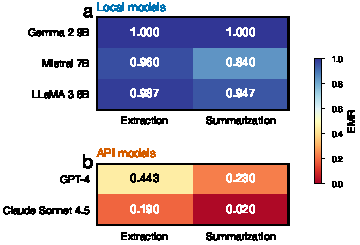
\includegraphics[width=0.65\columnwidth]{figures/fig_emr_heatmap.pdf}
  \caption{\textbf{Exact match rates per deployment stack under greedy decoding reveal a four-fold local--API gap.}
  Heatmap of EMR \DIFdelbeginFL \DIFdelFL{for eight deployment stacks }\DIFdelendFL across extraction and \DIFdelbeginFL \DIFdelFL{summarization }\DIFdelendFL \DIFaddbeginFL \DIFaddFL{summarisation }\DIFaddendFL tasks under temperature~$=$~\DIFdelbeginFL \DIFdelFL{0.
  Local }\DIFdelendFL \DIFaddbeginFL \DIFaddFL{0
  for the eight deployment }\DIFaddendFL stacks \DIFaddbeginFL \DIFaddFL{measured on Tasks~1--2 with full coverage:
  three local stacks }\DIFaddendFL (\DIFdelbeginFL \DIFdelFL{top}\DIFdelendFL \DIFaddbeginFL \DIFaddFL{L-LLaMA3, L-Mistral, L-Gemma2}\DIFaddendFL ; blue)\DIFaddbeginFL \DIFaddFL{, the Together AI quasi-isolation probe (C-LLaMA3),
  and four API stacks (API-DeepSeek, API-GPT4, API-Claude, API-Perplexity; red).
  The fifth API stack (API-Gemini) is evaluated only on Tasks~3--4 (multi-turn and RAG) and therefore appears in Fig.~\ref{fig:multiturn} rather than here.
  Local stacks }\DIFaddendFL achieve EMR~$\geq$~0.840, with \DIFdelbeginFL \DIFdelFL{the Gemma~2 9B stack }\DIFdelendFL \DIFaddbeginFL \DIFaddFL{L-Gemma2 }\DIFaddendFL at a perfect 1.000.
  API-served stacks \DIFdelbeginFL \DIFdelFL{(bottom; red) }\DIFdelendFL range from 0.800 (\DIFdelbeginFL \DIFdelFL{DeepSeek}\DIFdelendFL \DIFaddbeginFL \DIFaddFL{API-DeepSeek}\DIFaddendFL ) to 0.010 (\DIFdelbeginFL \DIFdelFL{Perplexity}\DIFdelendFL \DIFaddbeginFL \DIFaddFL{API-Perplexity}\DIFaddendFL ).
  All values are computed under each stack's representative greedy condition (C1 for local stacks\DIFaddbeginFL \DIFaddFL{, C-LLaMA3, API-Claude, API-DeepSeek }\DIFaddendFL and \DIFdelbeginFL \DIFdelFL{Claude}\DIFdelendFL \DIFaddbeginFL \DIFaddFL{API-Perplexity}\DIFaddendFL ; C2 for \DIFdelbeginFL \DIFdelFL{GPT-4}\DIFdelendFL \DIFaddbeginFL \DIFaddFL{API-GPT4 because the OpenAI seed is advisory}\DIFaddendFL ; see Methods).
  }\label{fig:heatmap}
\end{figure}

%% --- Table 1: EMR with CIs (full width) ---
\begin{table*}[t]
\caption{\textbf{Exact match rate per deployment stack under greedy decoding, with 95\% bootstrap confidence intervals.}
Each row identifies a stack by its weights and provider/infrastructure class; full tuples (weights, provider, serving infrastructure, API layer) are listed in Methods~\ref{subsec:models}.
For local stacks, values reflect the fixed-seed condition (C1); for GPT-4, the variable-seed greedy condition (C2); for Claude, C1 (no seed parameter supported).
Bootstrap: 10\DIFaddbeginFL {\DIFaddendFL ,\DIFaddbeginFL }\DIFaddendFL 000 resamples, percentile method.
$n$~$=$~number of abstracts per group.}\label{tab:main}
\footnotesize
\begin{tabular}{@{}llccc@{}}
\toprule
\textbf{Deployment stack (weights)} & \textbf{Class} & \textbf{$n$} & \textbf{Extraction EMR} & \textbf{Summarization EMR} \\
\midrule
Gemma 2 9B      & Local & 10 & 1.000\,[1.00,\,1.00] & 1.000\,[1.00,\,1.00] \\
LLaMA 3 8B      & Local & 30 & 0.987\,[0.96,\,1.00] & 0.947\,[0.89,\,0.99] \\
Mistral 7B      & Local & 10 & 0.960\,[0.88,\,1.00] & 0.840\,[0.72,\,0.96] \\
\midrule
DeepSeek Chat   & API   & 10 & 0.800 & 0.760 \\
GPT-4           & API   & 30 & 0.443\,[0.32,\,0.57] & 0.230\,[0.16,\,0.30] \\
Claude Sonnet 4.5 & API & 10 & 0.190\,[0.05,\,0.40] & 0.020\,[0.00,\,0.05] \\
Perplexity Sonar & API  & 10 & 0.100 & 0.010 \\
\midrule
\multicolumn{2}{l}{\textit{Local-stack average}} & & 0.982 & 0.929 \\
\multicolumn{2}{l}{\textit{API-stack average}}   & & 0.383 & 0.255 \\
\botrule
\end{tabular}
\normalsize
\end{table*}

%% --- Figure 2: Multi-turn + RAG (full width) ---
\begin{figure*}[t]
  \centering
  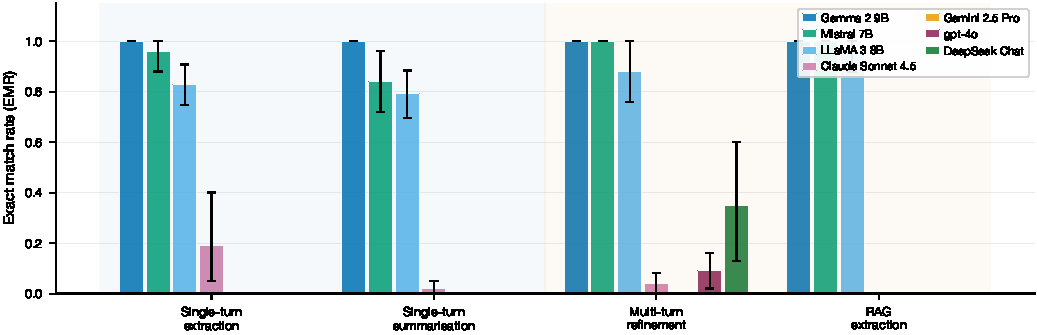
\includegraphics[width=0.78\textwidth]{figures/fig_multiturn_comparison.pdf}
  \caption{\textbf{Complex interaction regimes amplify the local--API reproducibility gap across deployment stacks.}
  EMR under greedy decoding (C1, $t$~$=$~0) for \DIFdelbeginFL \DIFdelFL{five deployment }\DIFdelendFL \DIFaddbeginFL \DIFaddFL{the local }\DIFaddendFL stacks \DIFaddbeginFL \DIFaddFL{(Gemma~2, Mistral, LLaMA~3) and four API stacks (Claude Sonnet~4.5, Gemini~2.5 Pro, gpt-4o, and DeepSeek Chat) }\DIFaddendFL across four scenarios:
  single-turn extraction, single-turn \DIFdelbeginFL \DIFdelFL{summarization}\DIFdelendFL \DIFaddbeginFL \DIFaddFL{summarisation}\DIFaddendFL , multi-turn refinement, and RAG extraction.
  Local stacks \DIFdelbeginFL \DIFdelFL{(Gemma~2, Mistral, LLaMA~3) }\DIFdelendFL maintain EMR~$\geq$~0.880 across all scenarios.
  \DIFdelbeginFL \DIFdelFL{Both }\DIFdelendFL \DIFaddbeginFL \DIFaddFL{All four }\DIFaddendFL API stacks \DIFaddbeginFL \DIFaddFL{exhibit low EMR on multi-turn refinement
  }\DIFaddendFL (Claude \DIFdelbeginFL \DIFdelFL{Sonnet}\DIFdelendFL \DIFaddbeginFL \DIFaddFL{EMR}\DIFaddendFL ~\DIFdelbeginFL \DIFdelFL{4.5 and }\DIFdelendFL \DIFaddbeginFL \DIFaddFL{$=$~0.040, }\DIFaddendFL Gemini~\DIFdelbeginFL \DIFdelFL{2.5 Pro}\DIFdelendFL \DIFaddbeginFL \DIFaddFL{$=$~0.010, gpt-4o~$=$~0.090 }[\DIFaddFL{0.02,\,0.16}]\DIFaddFL{, DeepSeek~$=$~0.350 }[\DIFaddFL{0.13,\,0.60}]\DIFaddendFL )\DIFdelbeginFL \DIFdelFL{exhibit near-zero EMR}\DIFdelendFL ,
  with the Claude stack achieving 0.000 for RAG (50 runs, zero exact matches).
  \DIFaddbeginFL \DIFaddFL{The gpt-4o and DeepSeek multi-turn results (10 abstracts $\times$ 5 repetitions each) were added in revision per reviewer request R3.3 and do not have RAG coverage; gpt-4o and DeepSeek bars therefore appear only in the multi-turn panel.
  }\DIFaddendFL Error bars: 95\% bootstrap CIs.
  }\label{fig:multiturn}
\end{figure*}

%% --- Figure 3: Three-level radar (single column) ---
\begin{figure}[t]
  \centering
  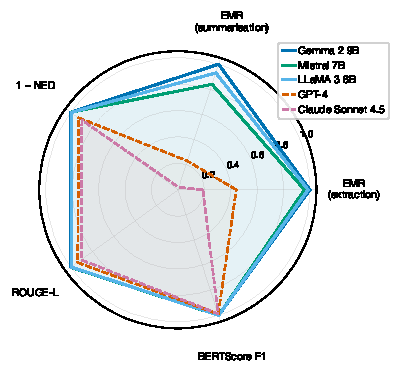
\includegraphics[width=0.6\columnwidth]{figures/fig_three_level_radar.pdf}
  \caption{\textbf{API non-determinism is textual, not semantic.}
  Three-level reproducibility profiles under greedy decoding.
  Local models (solid lines) occupy the outer region across all metrics.
  API models (dashed lines) show pronounced deficits in EMR and NED
  while maintaining BERTScore F1~$>$~0.97 (hidden non-determinism).
  Axes: EMR (extraction), EMR (\DIFdelbeginFL \DIFdelFL{summarization}\DIFdelendFL \DIFaddbeginFL \DIFaddFL{summarisation}\DIFaddendFL ), 1$-$NED, ROUGE-L, BERTScore F1.
  }\label{fig:radar}
\end{figure}

%% --- Figure 4: Temperature effect (full width) ---
\begin{figure*}[t]
  \centering
  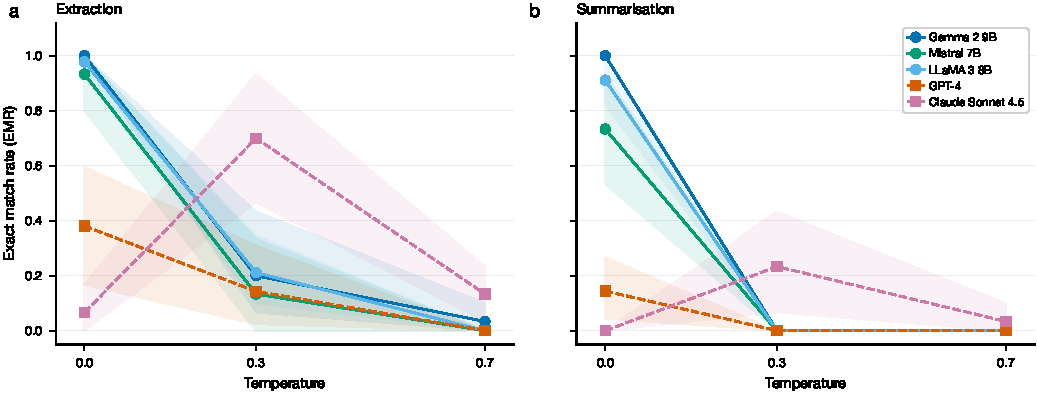
\includegraphics[width=0.88\textwidth]{figures/fig_temp_effect.pdf}
  \caption{\textbf{Temperature paradox: greedy decoding is not greedy for API models.}
  EMR versus temperature for five models (three local, two API).
  \textbf{a,}~Extraction. \textbf{b,}~Summarization.
  Local models (solid lines) show the expected monotonic decline from near-perfect EMR at $t$~$=$~0.
  API models (dashed lines) start from an already-low baseline.
  Claude Sonnet~4.5 (red dashed) exhibits a non-monotonic anomaly:
  extraction EMR \emph{increases} from 0.067 at $t$~$=$~0 to 0.700 at $t$~$=$~0.3.
  }\label{fig:temperature}
\end{figure*}

%% --- Figure 5: Visual abstract / pipeline (full width) ---
\begin{figure*}[t]
  \centering
  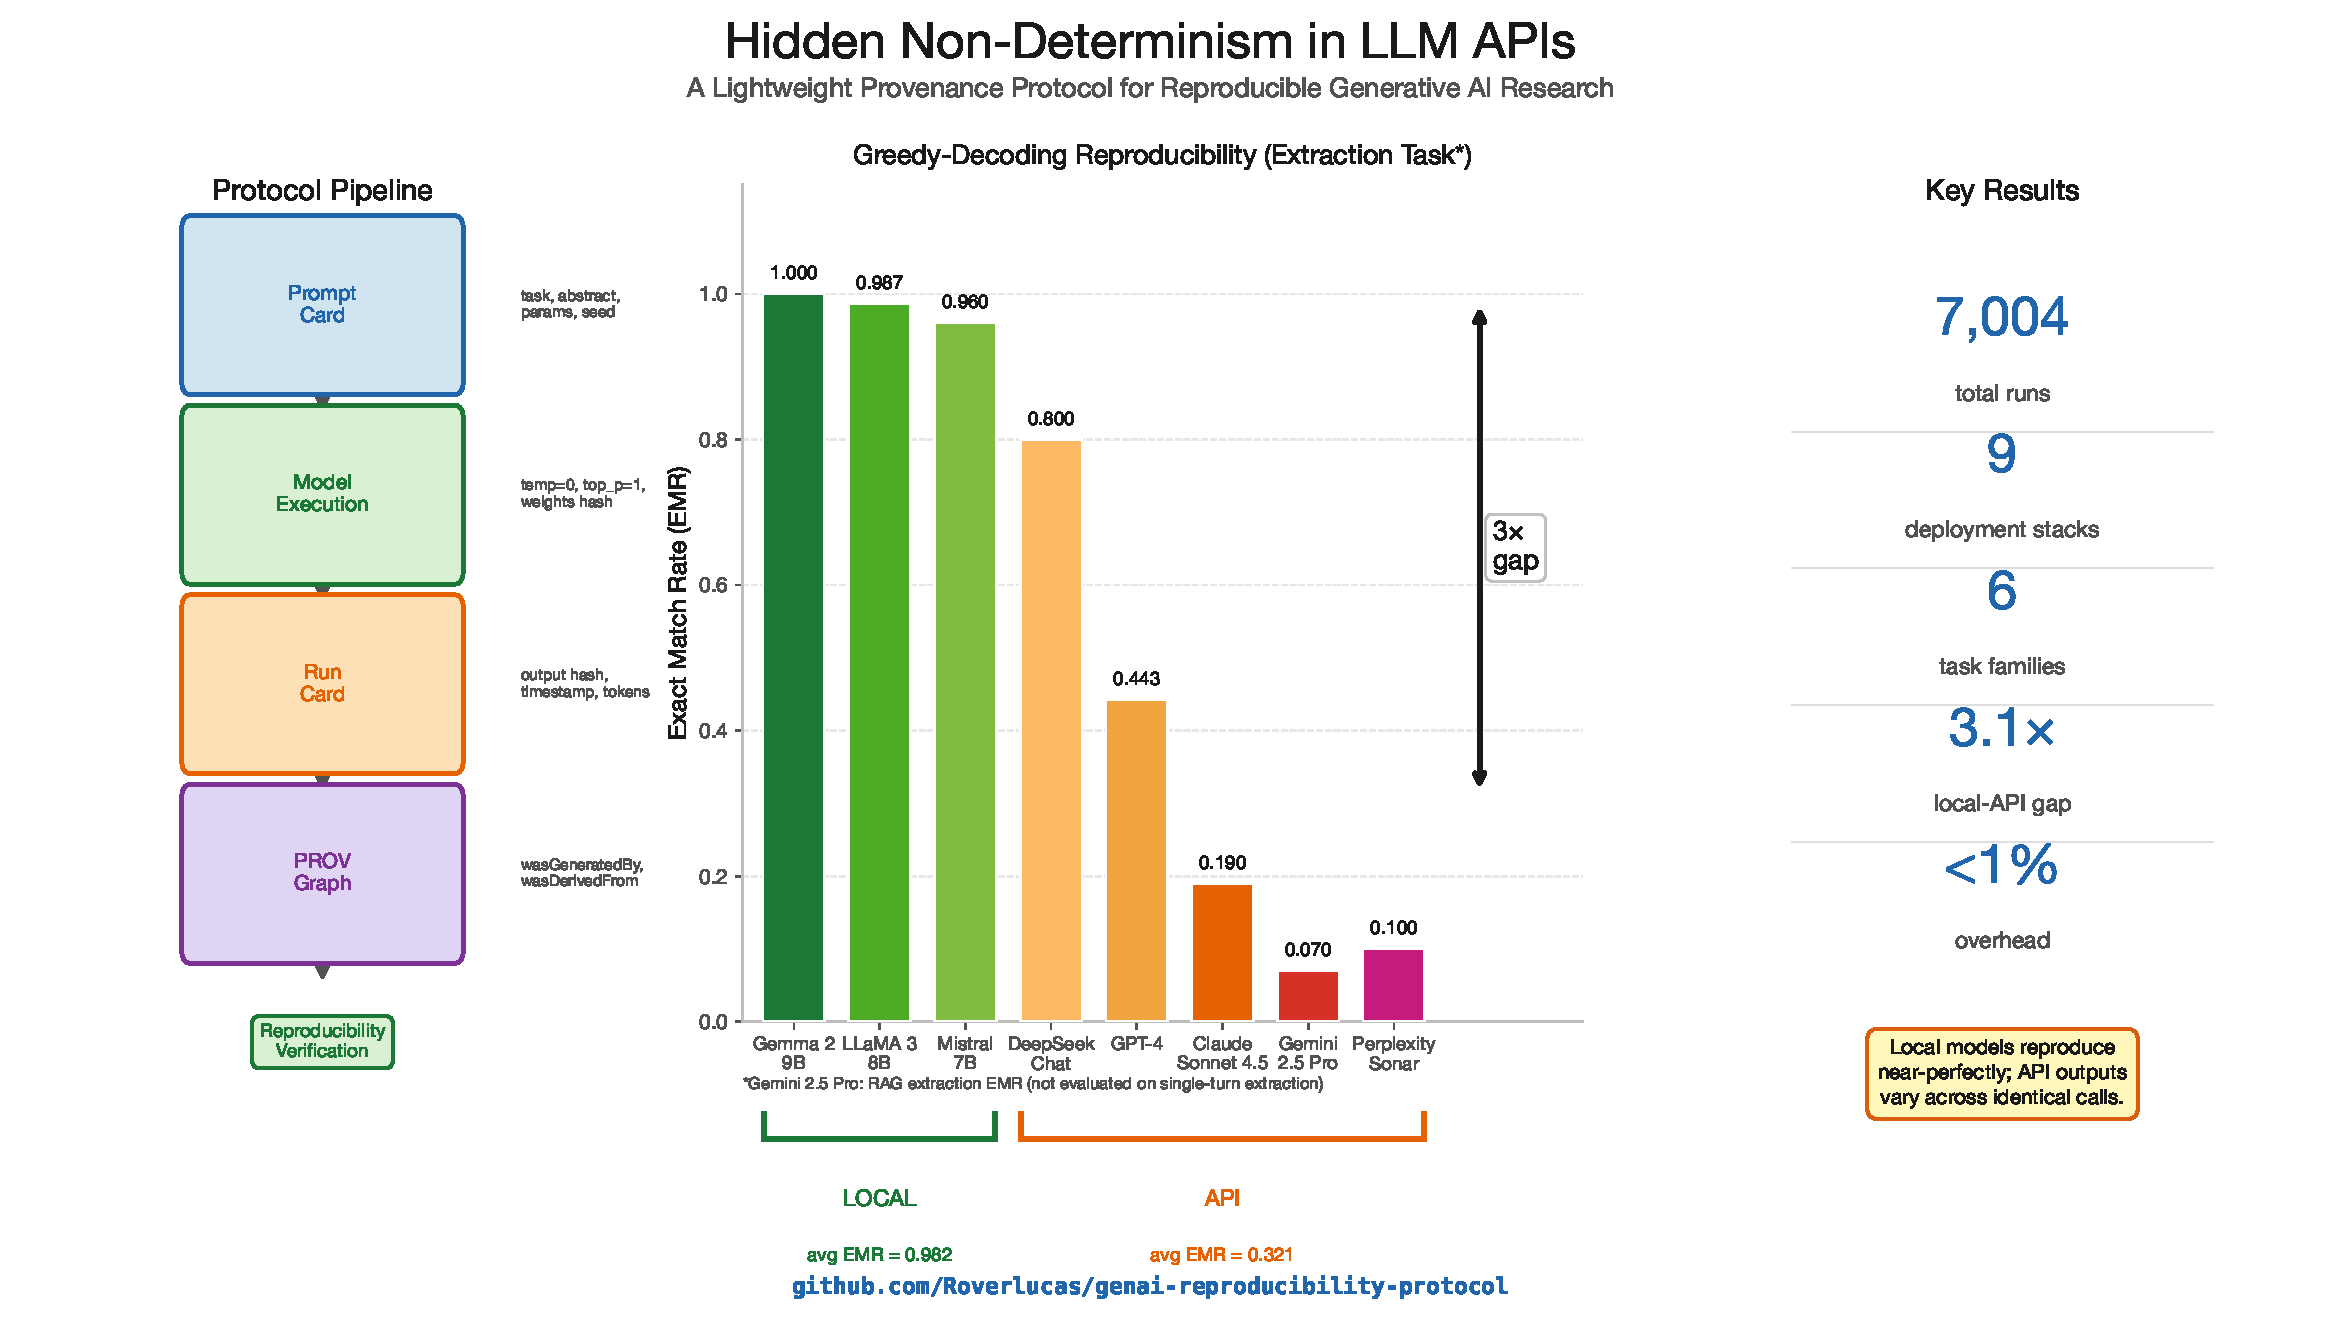
\includegraphics[width=0.82\textwidth]{figures/fig_visual_abstract.pdf}
  \caption{\textbf{Study overview and provenance protocol.}
  \textbf{Left:} The provenance pipeline, from Prompt Card creation through Run Card logging
  and W3C PROV graph generation.
  \textbf{Centre:} EMR under greedy decoding for eight deployment stacks,
  illustrating the local--API reproducibility gap
  (local stacks green, EMR~$\geq$~0.840; API stacks red, EMR~$\leq$~0.800).
  \textbf{Right:} Key statistics: \DIFdelbeginFL \DIFdelFL{4}\DIFdelendFL \DIFaddbeginFL \DIFaddFL{7}{\DIFaddendFL ,\DIFdelbeginFL \DIFdelFL{104 }\DIFdelendFL \DIFaddbeginFL }\DIFaddFL{004 }\DIFaddendFL experiments, 9 deployment stacks, \DIFdelbeginFL \DIFdelFL{7 execution environments}\DIFdelendFL \DIFaddbeginFL \DIFaddFL{6 task families}\DIFaddendFL ,
  \DIFdelbeginFL \DIFdelFL{4 tasks}\DIFdelendFL \DIFaddbeginFL \DIFaddFL{3.1$\times$ local--API gap (balanced subsample)}\DIFaddendFL , $<$1\% protocol overhead.
  }\label{fig:overview}
\end{figure*}

%DIF > % --- Box 1: Concrete examples of divergent outputs (T12) ---
\DIFaddbegin \begin{figure*}[t]
\centering
\DIFaddFL{\fbox{\begin{minipage}{0.94\textwidth}
\small
\textbf{Box~1\quad Concrete examples of divergent outputs under identical prompts and parameters.}

All examples below are taken from logged Run Cards in our public repository. For each example the prompt, decoding parameters (\texttt{temperature}~$=$~0, \texttt{seed}~$=$~42), model identifier, and resolved snapshot are byte-identical across runs; only the resulting output differs. Differences within \texttt{key\_result}, \texttt{method}, and \texttt{benchmark} are highlighted in red.

\medskip
\noindent\textbf{Example 1 (textual divergence; \texttt{benchmark} field).}
GPT-4 (gpt-4-0613), structured extraction, abstract 001 (Vaswani et al., 2017).
\begin{itemize}
\item[\DIFaddFL{Run~A:}] \texttt{"benchmark": "WMT 2014 English-to-German translation task\textcolor{red}{\textbf{,}} WMT 2014 English-to-French translation task"}
\item[\DIFaddFL{Run~B:}] \texttt{"benchmark": "WMT 2014 English-to-German translation task \textcolor{red}{\textbf{and}} WMT 2014 English-to-French translation task"}
\end{itemize}
The two strings denote the same evaluation set but are bitwise distinct; an automated pipeline that splits on commas would see two benchmarks in Run~A and one in Run~B.

\medskip
\noindent\textbf{Example 2 (substantive divergence; \texttt{key\_result} field).}
Claude Sonnet~4.5 (\texttt{claude-sonnet-4-5-20250929}), RAG extraction, abstract 001.
\begin{itemize}
\item[\DIFaddFL{Run~A:}] \texttt{"key\_result": "Achieved 28.4 BLEU on WMT 2014 English-to-German $\ldots$ and 41.8 BLEU on WMT 2014 English-to-French $\ldots$ \textcolor{red}{\textbf{with superior parallelizability and reduced training time (3.5 days on 8 GPUs)}}"}
\item[\DIFaddFL{Run~B:}] \texttt{"key\_result": "Achieved 28.4 BLEU on WMT 2014 English-to-German $\ldots$ and 41.8 BLEU on WMT 2014 English-to-French $\ldots$ \textcolor{red}{\textbf{after training for 3.5 days on eight GPUs; also successfully generalized to English constituency parsing}}"}
\end{itemize}
The two outputs report the same headline numbers but populate \texttt{key\_result} with different supporting facts: a downstream meta-analysis that sub-classifies findings by ``parallelizability'' versus ``generalisation to parsing'' would assign these two runs to different categories.

\medskip
\noindent\textbf{Example 3 (substantive divergence; \texttt{method} field).}
Claude Sonnet~4.5, RAG extraction, abstract 001 (same group as Example~2).
\begin{itemize}
\item[\DIFaddFL{Run~A:}] \texttt{"method": "Transformer architecture based entirely on attention mechanisms, \textcolor{red}{\textbf{without recurrent or convolutional layers}}, connecting encoder and decoder $\ldots$"}
\item[\DIFaddFL{Run~B:}] \texttt{"method": "The Transformer architecture using only attention mechanisms to connect encoder and decoder, \textcolor{red}{\textbf{dispensing with recurrent and convolutional neural networks entirely}}"}
\end{itemize}
The architectural claim is preserved, but the wording is fully reformulated; downstream tools that match \texttt{method} strings exactly would treat these as different methods.
\end{minipage}}
}\caption{\textbf{\DIFaddFL{Concrete examples of divergent outputs under identical prompts, parameters, and resolved snapshots.}}
\DIFaddFL{Examples~1--3 are drawn from the public Run Card repository.
Highlighting marks the diverging spans.}}\label{box:examples}
\end{figure*}


\DIFaddend %%=============================================================%%
%% DISCUSSION
%%=============================================================%%
\section{Discussion}\label{sec:discussion}

Our findings reveal a pervasive and previously invisible reproducibility gap in LLM-based research.
Under the settings that API documentation presents as deterministic (temperature zero, fixed seed), API-served models fail to reproduce their own outputs approximately four out of five times.
This gap persists across five independent providers, extends to multi-turn and RAG workflows, and survives rigorous statistical correction.
The immediate implication is that a substantial portion of published research relying on API-based LLMs may contain non-reproducible results without the authors' knowledge, a concern amplified by the growing use of LLMs in peer review\cite{thakkar2026llm}, hypothesis generation\cite{xin2025agentic}, and agentic pipelines where non-determinism compounds at every step.

Prior work documented LLM non-determinism in isolated settings: inconsistent NLP benchmark outputs\cite{chen2023chatgpt}, failure of ``deterministic'' API settings\cite{atil2024nondeterminism}, and non-deterministic code generation\cite{ouyang2024nondeterminism}.
Our study advances beyond these observations by systematically comparing local versus API deployments across five providers, extending measurements to multi-turn and RAG workflows, and providing a causal attribution framework that distinguishes infrastructure complexity from cloud deployment.

The Together AI quasi-isolation result provides a key mechanistic insight: because the same model architecture achieves near-local reproducibility via a different cloud API, the non-determinism observed in GPT-4, Claude, and Gemini is attributable to production serving complexity rather than cloud deployment itself.
This suggests that reproducibility is a design choice that providers could address through deterministic execution modes or transparent documentation, rather than an inherent limitation.
Documenting temperature zero as ``deterministic'' without disclosing infrastructure-level variation creates a false sense of reproducibility that may be more damaging than openly acknowledged stochasticity.

A direct consequence is that the \emph{deployment stack}, not the abstract model, is the carrier of variation in LLM-based research.
The same LLaMA~3 8B weights yield near-perfect reproducibility under one stack (local Ollama) and substantially lower reproducibility when wrapped in a different cloud-serving stack; conversely, two different sets of weights served by stacks of comparable complexity (GPT-4 and Claude) show qualitatively similar reproducibility profiles.
This reframes the methodological recommendation: research and regulatory documentation that names ``the model'' should instead identify the deployment stack as a tuple of weights, provider, serving infrastructure, and API layer.
Without that specification, ``using GPT-4'' or ``using Claude'' is under-specified for reproducibility purposes, because the same nominal model served through different stacks can produce materially different outputs and stability profiles.

These findings also have regulatory implications.
The EU AI Act\cite{euaiact2024} requires traceability for high-risk AI systems, and the NIST AI RMF\cite{nist2023ai} \DIFdelbegin \DIFdel{emphasizes }\DIFdelend \DIFaddbegin \DIFadd{emphasises }\DIFaddend transparency; hidden non-determinism directly undermines both.
Ethical guidelines for LLM use in academic writing\cite{porsdam2024ethics} similarly assume that documented configurations produce predictable outputs, an assumption our results show to be unwarranted.

Although the semantic preservation we observe (BERTScore F1~$>$~0.97) suggests that output quality is not corrupted, our field-level analysis shows that even ``semantically equivalent'' outputs differ in conclusion-relevant fields; the 78\% non-match rate under ``deterministic'' settings represents a serious obstacle for regulatory submissions, systematic reviews, and automated pipelines.

The provenance protocol we provide offers a practical path forward.
Grounded in W3C PROV\cite{w3cprov2013} and adding less than 1\% overhead (Extended Data Table~6), it creates auditable records linking every output to its generation context.
Its key property is \emph{differential diagnosis}: when all hashes match except the output hash, the divergence is automatically attributed to the generation process, a result \DIFdelbegin \DIFdel{confirmed across all 4,104 }\DIFdelend \DIFaddbegin \DIFadd{verified by the protocol-minimality ablation across 1}{\DIFadd{,}}\DIFadd{864 }\DIFaddend runs (Supplementary Section~\DIFdelbegin \DIFdel{S4) }\DIFdelend \DIFaddbegin \DIFadd{S6) and consistent with the full 4}{\DIFadd{,}}\DIFadd{104-run analysis}\DIFaddend .
This implements what recent editorials have advocated\cite{editorial2024framework} and extends Model Cards\cite{mitchell2019model} and Datasheets\cite{gebru2021datasheets} to the inference layer.
We propose a minimum reporting standard (model identity, parameters, reproducibility metrics, deployment mode, and output hashes) that our protocol automates at negligible cost (Supplementary Information).

Our study has several limitations.
It covers \DIFdelbegin \DIFdel{eight models across four tasks but excludes }\DIFdelend \DIFaddbegin \DIFadd{nine deployment stacks across six task families (structured extraction, scientific summarisation, multi-turn refinement, retrieval-augmented generation, }\DIFaddend code generation, \DIFdelbegin \DIFdel{mathematical reasoning}\DIFdelend \DIFaddbegin \DIFadd{and mathematical reasoning), but excludes creative writing}\DIFaddend , \DIFdelbegin \DIFdel{and creative writing}\DIFdelend \DIFaddbegin \DIFadd{free-form long-form generation, and non-English content; future work should extend the protocol to those domains}\DIFaddend .
Input data \DIFaddbegin \DIFadd{for the original Tasks~1--4 }\DIFaddend comprises 30 English-language AI/ML abstracts; \DIFdelbegin \DIFdel{other languages and domains may show amplified effects.
}\DIFdelend \DIFaddbegin \DIFadd{the revision extends to standard public benchmarks (HumanEval, GSM8K) and to 10 PubMed PM\textsubscript{2.5} abstracts as an out-of-AI/ML probe, with the same qualitative pattern observed in each.
The original }\DIFaddend GPT-4 experiments used the \texttt{gpt-4-0613} snapshot\DIFdelbegin \DIFdel{; newer versions may differ , though the infrastructure-level mechanisms we identify are general.
Multi-turn and RAG experiments include only two API providers; extending to others would }\DIFdelend \DIFaddbegin \DIFadd{, which may differ from current production behaviour; we partly mitigated this by running a current-snapshot subset (}\texttt{\DIFadd{gpt-4o-2024-11-20}}\DIFadd{) on the multi-turn extension, on HumanEval and GSM8K, and on the PubMed PM\textsubscript{2.5} probe, confirming that the qualitative local--API pattern persists at a current snapshot.
The multi-turn refinement task now covers four API stacks (Claude, Gemini, gpt-4o, DeepSeek), but RAG coverage remains restricted to Claude and Gemini and extending the RAG regime to additional providers would further }\DIFaddend strengthen generality.
Sample sizes (10--30 \DIFdelbegin \DIFdel{abstracts per model }\DIFdelend \DIFaddbegin \DIFadd{problems per model per revision task}\DIFaddend ) are well-powered for the large observed effects ($d$~$>$~1.6) but may miss subtler phenomena.
\DIFaddbegin \DIFadd{The applied-impact validation in §\ref{subsec:pubmed} uses two independent LLM-as-judge providers (Claude Opus 4.7 and gpt-4o) rather than human raters; while the cross-provider design directly addresses the standard ``LLM-on-LLM'' bias concern and the convergence of both judges on the majority verdict is consistent with substantive divergence, a multi-rater human validation against a domain-expert silver standard on a larger sample is the natural next methodological step and is in preparation as a dedicated follow-up paper.
}\DIFaddend 

\DIFdelbegin \DIFdel{Indeed, preliminary evidence }\DIFdelend \DIFaddbegin \DIFadd{The Together AI quasi-isolation result also has scope limits that we wish to make explicit.
The probe demonstrates that cloud deployment is }\emph{\DIFadd{not a sufficient cause}} \DIFadd{of LLM non-determinism: an open-weight model served by a cloud endpoint can recover near-local reproducibility.
We do }\emph{\DIFadd{not}} \DIFadd{claim, and the result does not warrant claiming, that the proprietary stacks behind GPT-4, Claude, and Gemini could achieve the same level of reproducibility under their current production-infrastructure design constraints; their stacks are closed and we cannot run the symmetric ``same-weights, two-stacks'' comparison against them.
It remains possible that throughput, multi-tenancy, and latency requirements at the scale of these providers make near-local reproducibility infeasible without architectural changes.
The Together AI result is therefore offered as evidence for the }\emph{\DIFadd{weaker}} \DIFadd{claim---that the cause of API non-determinism is production serving infrastructure complexity rather than the cloud medium itself---and as a partial existence proof that closed-source providers retain the option to publish reproducibility-prioritised execution modes.
}

\DIFadd{Evidence }\DIFaddend from an applied domain \DIFdelbegin \DIFdel{suggests }\DIFdelend \DIFaddbegin \DIFadd{confirms }\DIFaddend that the effects reported here have direct consequences for scientific conclusions.
In a companion study applying six LLMs to a 500-abstract corpus of epidemiological studies on fine particulate matter (PM\DIFdelbegin \DIFdel{$_{2.5}$}\DIFdelend \DIFaddbegin \DIFadd{\textsubscript{2.5}}\DIFaddend ) and respiratory health\cite{rover2026evidence}, we find that extraction EMR under identical deterministic settings drops to 0.050 (Claude), 0.150 (GPT-4.1), and 0.200 (Gemini~2.5 Pro) \DIFdelbegin \DIFdel{---consistent }\DIFdelend \DIFaddbegin \DIFadd{on the full 500-abstract corpus---consistent }\DIFaddend with, and in some cases worse than, the values reported here \DIFaddbegin \DIFadd{on the 10-abstract probe (where Claude EMR collapses further to 0.010 because the smaller corpus concentrates the within-abstract variance; the two values therefore quantify the same phenomenon at different sampling scales)}\DIFaddend .
Critically, a meta-analytic propagation analysis reveals that up to 23 study-level effect estimates---each representing a distinct epidemiological finding on air pollution and respiratory outcomes---appear or disappear from the evidence base depending solely on which run of the LLM is used.
This confirms that the hidden non-determinism documented in the present study is not confined to AI/ML benchmarks but propagates into applied health research where it can alter the composition of evidence available for clinical guidelines and regulatory decisions.

\DIFdelbegin \DIFdel{In summary, the }\DIFdelend \DIFaddbegin \DIFadd{The }\DIFaddend ``deterministic'' settings offered by major LLM API providers do not deliver determinism in practice, creating a hidden reproducibility gap that spans five providers, persists across multi-turn and RAG workflows, and remains invisible because semantic equivalence \DIFdelbegin \DIFdel{masks textual divergence}\DIFdelend \DIFaddbegin \DIFadd{under aggregate metrics masks textual---and sometimes substantive---divergence}\DIFaddend .
Our quasi-isolation experiment attributes the cause to production infrastructure complexity rather than cloud deployment itself.
The lightweight provenance protocol we provide, grounded in W3C PROV and requiring less than 1\% overhead, makes this variation visible, auditable, and attributable, offering an actionable path toward reproducible LLM-based research.
As large language models become embedded in clinical decision support, environmental monitoring, engineering design, and automated data analysis, the inability to reproduce a model's output is not merely an academic inconvenience but a threat to the trustworthiness of systems that depend on it.
Without explicit provenance tracking, the reliability of any LLM-based pipeline built on API inference cannot be assumed; it must be measured, documented, and continuously monitored.


%%=============================================================%%
%% METHODS
%%=============================================================%%
\section{Methods}\label{sec:methods}

\subsection{Protocol design}\label{subsec:protocol}

The provenance protocol addresses the question: what is the minimum metadata needed per generative AI run to enable reproducibility assessment, auditing, and provenance tracking?
The FAIR principles\cite{wilkinson2016fair} provide a foundation for data stewardship, yet no standard exists for documenting the full context of generative AI outputs.
Existing experiment-tracking tools such as MLflow\cite{zaharia2018accelerating} were designed for training pipelines and numerical metrics, not for inference-time text-generation provenance.
Data leakage analysis across 17 ML fields\cite{kapoor2023leakage} underscores the urgency of structured documentation.
\DIFdelbegin \DIFdel{It }\DIFdelend \DIFaddbegin 

\textbf{\DIFadd{Scope: client-side observability.}}
\DIFadd{The protocol is designed for any researcher who calls an LLM, regardless of whether the underlying stack is open-source or proprietary.
It documents what is }\emph{\DIFadd{observable from the client side}}\DIFadd{: the request payload, the resolved model identifier returned by the API, response headers, the API response identifier, latency, and the input/output text together with their cryptographic hashes.
It does }\emph{\DIFadd{not}} \DIFadd{require provider-side weight hashes, full infrastructure disclosure, or kernel-level traces, none of which are accessible for closed-source stacks.
This client-side scope is intentional: it enables }\emph{\DIFadd{differential diagnosis}} \DIFadd{for any researcher.
When the same prompt and parameters yield different outputs across runs, the Run Card records evidence that the divergence arose at the generation step rather than from a change in inputs, parameters, or environment.
For proprietary APIs in particular, the protocol creates the audit trail that providers' opacity would otherwise make impossible.
The protocol is therefore not restricted to open-source stacks; it is the minimum machinery that closes the audit loop on }\emph{\DIFadd{any}} \DIFadd{deployment stack.
It }\DIFaddend comprises four components.

\textbf{Prompt Cards} are versioned documentation artifacts capturing design rationale and metadata for prompt templates, including SHA-256 hash, version, task category, assumptions, limitations, and target models.
The concept extends Model Cards\cite{mitchell2019model} and Datasheets for Datasets\cite{gebru2021datasheets} to the prompt layer.

\textbf{Run Cards} capture the complete execution context of a single generative AI run through 24 core fields \DIFdelbegin \DIFdel{organized }\DIFdelend \DIFaddbegin \DIFadd{organised }\DIFaddend into five groups: identification (run ID, prompt hash, prompt text), model context (name, version, weights hash), parameters (temperature, seed, decoding strategy, parameters hash), input/output (text and SHA-256 hashes), and execution metadata (environment fingerprint, timestamps, duration, logging overhead).
For API models, optional extension fields capture provider-specific metadata: API request ID, response headers, resolved model version, and a \texttt{seed\_status} field distinguishing between seeds that were ``sent'', ``logged-only'' (recorded for protocol parity but not transmitted, as with Claude), or ``not-supported''.

\textbf{W3C PROV integration.}
Each experimental group is translated into a PROV-JSON document\cite{w3cprov2013} expressing generation provenance as a directed graph of entities (Prompt, InputText, ModelVersion, InferenceParameters, Output), activities (RunGeneration), and agents (Researcher, SystemExecutor).
The formal semantics of PROV enable automated traversal and comparison, identifying the exact factor that differs between non-identical outputs without custom parsing.

\textbf{Reproducibility checklist.}
A 15-item checklist \DIFdelbegin \DIFdel{organized }\DIFdelend \DIFaddbegin \DIFadd{organised }\DIFaddend into four categories (Prompt Documentation, Model and Environment, Execution and Output, Provenance) enables self-assessment.

We formally define the protocol as a tuple $\mathcal{P} = (\mathit{PC}, \mathit{RC}, G, \mathit{CL})$ and prove an \emph{audit completeness} property: for 10 defined audit questions, every question is answerable if and only if all field groups are populated.
An ablation analysis confirms \emph{minimality}: removing any field group renders at least one question unanswerable (Extended Data Table~6).


\subsection{Unit of analysis: deployment stacks}\label{subsec:stacks}

We define a \emph{deployment stack} as the tuple (model weights, provider, serving infrastructure, API layer).
The same model weights served by two different stacks constitute two distinct experimental objects for reproducibility purposes, since each component of the tuple can independently introduce variation: weights through quantisation, provider through routing and post-processing, serving infrastructure through tensor parallelism, mixed-precision accumulation, FlashAttention kernels, dynamic batching, and speculative decoding (Methods~\ref{subsec:sources}), and the API layer through prompt templating, response truncation, and resolved-version aliasing.
This conceptual frame resolves the question of whether observed differences arise from the model itself or from how it is served.
The Together AI quasi-isolation probe (Methods~\ref{subsec:models}) provides direct evidence: the same LLaMA~3 8B weights served via local Ollama versus Together AI's cloud endpoint produce stacks with \DIFdelbegin \DIFdel{markedly }\DIFdelend \DIFaddbegin \DIFadd{measurably }\DIFaddend different reproducibility profiles\DIFdelbegin \DIFdel{only at the lower-precision boundary, while preserving near-local EMR overall}\DIFdelend \DIFaddbegin \DIFadd{, even when the underlying weights are identical}\DIFaddend .
We therefore report results per \emph{stack} rather than per \emph{model}.
Throughout the manuscript, identifiers such as ``GPT-4'' refer to the full deployment stack (gpt-4-0613 / OpenAI / production cluster / Chat Completions API) at the time of measurement, not to a provider-independent model abstraction.


\subsection{Deployment stacks evaluated}\label{subsec:models}

We evaluate nine deployment stacks across three paradigms.
Each stack is identified by the tuple (model weights / provider / serving infrastructure / API layer).

\textbf{Local stacks} (Ollama v0.15.5, Apple M4, 24\,GB unified memory, macOS~14.6, Python~3.14.3):
\textbf{L-LLaMA3} = (LLaMA~3 8B Q4\_0\cite{grattafiori2024llama3} / local Ollama / single-GPU Apple M4 / Ollama \texttt{/api/generate});
\textbf{L-Mistral} = (Mistral~7B Q4\_0\cite{jiang2023mistral} / local Ollama / single-GPU Apple M4 / Ollama \texttt{/api/generate});
\textbf{L-Gemma2} = (Gemma~2 9B Q4\_0\cite{team2024gemma} / local Ollama / single-GPU Apple M4 / Ollama \texttt{/api/generate}).
Weights hashes recorded via the Ollama API.

\textbf{API-served stacks} (full stack opaque; reference local pair available only for L-LLaMA3):
\textbf{API-GPT4} = (\texttt{gpt-4-0613}\cite{achiam2023gpt4} / OpenAI / production cluster / Chat Completions API);
\textbf{API-Claude} = (\texttt{claude-sonnet-4-5-20250929}\cite{anthropic2024claude} / Anthropic / production cluster / Messages API via urllib);
\textbf{API-Gemini} = (\texttt{gemini-2.5-pro-preview-05-06}\cite{reid2024gemini15} / Google / production cluster / AI Studio REST API via urllib);
\textbf{API-DeepSeek} = (DeepSeek Chat / DeepSeek / production cluster / OpenAI-compatible API);
\textbf{API-Perplexity} = (Sonar / Perplexity / production cluster + retrieval / Perplexity API).

\textbf{Quasi-isolation probe stack}:
\textbf{C-LLaMA3} = (LLaMA~3 8B \DIFaddbegin \DIFadd{Q4\_0 (}\DIFaddend INT4\DIFaddbegin \DIFadd{)}\DIFaddend \cite{grattafiori2024llama3} / Together AI / multi-GPU cloud / OpenAI-compatible API), pairing with L-LLaMA3 to isolate cloud serving from production-infrastructure complexity. \DIFaddbegin \DIFadd{Both L-LLaMA3 and C-LLaMA3 use the same Q4\_0 INT4 quantisation of the LLaMA~3 8B weights; the only difference is the serving infrastructure.
}\DIFaddend 


\subsection{Tasks}\label{subsec:tasks}

\DIFdelbegin \DIFdel{Four tasks }\DIFdelend \DIFaddbegin \DIFadd{Six task families }\DIFaddend spanning the output-structure spectrum\DIFdelbegin \DIFdel{:
}\DIFdelend \DIFaddbegin \DIFadd{.
The first four were evaluated in the original analysis:
}\DIFaddend \textbf{Task~1, Scientific \DIFdelbegin \DIFdel{summarization}\DIFdelend \DIFaddbegin \DIFadd{summarisation}\DIFaddend :} produce a three-sentence summary of a scientific abstract.
\textbf{Task~2, Structured extraction:} extract five fields (objective, method, key\_result, model\_or\_system, benchmark) as JSON.
\textbf{Task~3, Multi-turn refinement:} three-turn dialogue (extract, receive feedback, refine).
\textbf{Task~4, RAG extraction:} structured extraction with a prepended retrieved context passage.

\DIFaddbegin \DIFadd{Two additional task families were added in revision:
}\textbf{\DIFadd{Task~5, Code generation (HumanEval):}} \DIFadd{30 problems sampled in a stratified manner from the 164-problem HumanEval benchmark\mbox{%DIFAUXCMD
\cite{chen2021humaneval}}\hskip0pt%DIFAUXCMD
, prompt format }\texttt{\DIFadd{prompt + ``\textbackslash n''}}\DIFadd{, output is the function body up to the first }\texttt{\DIFadd{return}} \DIFadd{block.
}\textbf{\DIFadd{Task~6, Math reasoning (GSM8K):}} \DIFadd{30 problems sampled from the GSM8K test split\mbox{%DIFAUXCMD
\cite{cobbe2021gsm8k}}\hskip0pt%DIFAUXCMD
, prompt format ``Question: \{q\}\textbackslash nAnswer:'', output is a free-form chain-of-thought derivation terminated by ``\#\#\#\# \{integer\}''.
A separate cross-domain probe (}\textbf{\DIFadd{Task~T14}}\DIFadd{, 10 PubMed abstracts on PM\textsubscript{2.5} and respiratory or cardiovascular health drawn from the companion paper's 500-abstract corpus\mbox{%DIFAUXCMD
\cite{rover2026evidence}}\hskip0pt%DIFAUXCMD
) was processed under Task~2's structured-extraction schema to test domain transfer outside AI/ML.
}


\DIFaddend \subsection{Input data}\label{subsec:input}

Thirty widely cited AI/ML abstracts (including Transformer, BERT, GPT-3, T5, and Chain-of-Thought\cite{vaswani2017attention,devlin2019bert,brown2020language,raffel2020exploring,wei2022chain}), varying in length (74--227 words) and technical complexity\DIFdelbegin \DIFdel{.
}\DIFdelend \DIFaddbegin \DIFadd{, are used for Tasks~1--4.
Revision tasks use established public benchmarks and a curated PubMed sample:
HumanEval problem identifiers (30 stratified) for Task~5, GSM8K test-split identifiers (30 sampled) for Task~6, and 10 PubMed abstracts with DOIs for Task~T14 (full lists and DOIs in Supplementary Section~S2 (original 30 abstracts) and Section~S11 (revision-batch identifiers)).
}\DIFaddend 


\subsection{Experimental conditions}\label{subsec:conditions}

Five conditions systematically vary reproducibility factors:
\textbf{C1} (fixed seed, greedy): $t$~$=$~0, seed~$=$~42, 5 repetitions;
\textbf{C2} (variable seeds, greedy): $t$~$=$~0, seeds~$=$~\{42, 123, 456, 789, 1024\}, 5 repetitions;
\textbf{C3} (temperature sweep): $t \in \{0.0, 0.3, 0.7\}$, 3 repetitions each.
\DIFaddbegin \DIFadd{In the original analysis, }\DIFaddend Tasks~1--2 \DIFaddbegin \DIFadd{were run }\DIFaddend under all conditions for five models with full coverage; Tasks~3--4 \DIFaddbegin \DIFadd{(multi-turn refinement and RAG extraction) were run }\DIFaddend under C1 for \DIFdelbegin \DIFdel{local models, Claude, and Gemini}\DIFdelend \DIFaddbegin \DIFadd{the local stacks, API-Claude, and API-Gemini}\DIFaddend .
DeepSeek and Perplexity: C1 only on Tasks~1--2 \DIFaddbegin \DIFadd{in the original analysis}\DIFaddend .
Together AI: C1 and C2 on Tasks~1--2.
Grand total \DIFaddbegin \DIFadd{for the original analysis}\DIFaddend : 4\DIFdelbegin \DIFdel{,}\DIFdelend \DIFaddbegin {\DIFadd{,}}\DIFaddend 104 logged runs across 9 deployments and 7 execution environments.
\DIFaddbegin \DIFadd{The Revision extensions paragraph below describes the additional Task~3 coverage (gpt-4o and DeepSeek), the new code/math/PubMed tasks, and the LLM-as-judge protocol added in revision.
}\DIFaddend 

\DIFaddbegin \textbf{\DIFadd{Revision extensions.}} \DIFadd{Following reviewer requests during the major revision (R3.3, R3.4, R3.6), three additional batches were logged under C1, each with five repetitions per problem and the same Run Card / Prompt Card provenance discipline as the original runs.
(a)~Task~5 (HumanEval, 30 problems) and Task~6 (GSM8K, 30 problems) were executed on the eight deployment stacks with full Tasks~1--2 coverage (L-LLaMA3, L-Mistral, L-Gemma2, C-LLaMA3, API-GPT4 with the gpt-4o-2024-11-20 snapshot, API-Claude, API-Gemini, API-DeepSeek), yielding 30~$\times$~5~$\times$~8 = 1}{\DIFadd{,}}\DIFadd{200 runs per task.
(b)~The multi-turn refinement task (Task~3) was extended to two additional API stacks (gpt-4o-2024-11-20 and API-DeepSeek) on 10 abstracts $\times$ 5 repetitions each, contributing 100 additional runs that complete the four-API-stack coverage shown in Fig.~\ref{fig:multiturn}.
(c)~Task~T14 (10 PubMed PM\textsubscript{2.5} abstracts under Task~2's extraction schema) was executed on the same eight deployment stacks (10~$\times$~5~$\times$~8 = 400 runs).
A blinded two-judge LLM-as-judge analysis on 30 sampled non-identical pairs (18 Claude Sonnet 4.5 + 12 GPT-4.1) from Task~T14 was run with Claude Opus 4.7 and gpt-4o as the two judges under three pre-registered criteria (direction, magnitude $\pm$20\%, CI overlap); full prompts and per-pair verdicts are in Supplementary Section~S12.
Revision total: 1}{\DIFadd{,}}\DIFadd{200 (HumanEval) + 1}{\DIFadd{,}}\DIFadd{200 (GSM8K) + 400 (PubMed PM\textsubscript{2.5}) + 100 (multi-turn extension) = 2}{\DIFadd{,}}\DIFadd{900 logged generative-AI runs, bringing the manuscript-wide total to 7}{\DIFadd{,}}\DIFadd{004 runs across 9 deployment stacks and 6 task families. An additional 60 LLM-as-judge calls (30 Claude Opus 4.7 + 30 gpt-4o, total cost USD~1.30, see Supplementary Section~S12, ``LLM-as-Judge Triangulation Protocol'') support the applied-impact triangulation but are reported separately as they belong to the validation layer rather than the primary experimental matrix.
}

\DIFaddend For API models, the seed parameter is advisory (OpenAI\cite{openai2024seed}), absent (Anthropic), or empirically insufficient (Gemini); greedy decoding does not guarantee determinism\cite{ouyang2024nondeterminism}.

\DIFaddbegin \textbf{\DIFadd{Anthropic seed handling.}}
\DIFadd{For completeness regarding C1 on Claude: the Anthropic Messages API does not accept a }\texttt{\DIFadd{seed}} \DIFadd{parameter, so no seed value is transmitted with any Claude request.
The Run Card nevertheless records }\texttt{\DIFadd{seed: 42}} \DIFadd{together with }\texttt{\DIFadd{seed\_status: "logged-only-not-sent-to-api"}}\DIFadd{, so that downstream audit tools can distinguish a seed that was }\emph{\DIFadd{requested}} \DIFadd{by the experimenter from one that was }\emph{\DIFadd{honoured}} \DIFadd{by the API (Supplementary Section~S4).
Claude is consequently evaluated under temperature~$=$~0, which Anthropic documents as selecting the most-probable next token at each step.
The non-determinism we observe for the Claude stack is therefore attributable to the production serving infrastructure rather than to seed variation.
}


\DIFaddend \subsection{Metrics}\label{subsec:metrics}

\textbf{Exact Match Rate (EMR):} fraction of all $\binom{n}{2}$ output pairs within a group that are character-identical.
\textbf{\DIFdelbegin \DIFdel{Normalized }\DIFdelend \DIFaddbegin \DIFadd{Normalised }\DIFaddend Edit Distance (NED):} Levenshtein distance\cite{levenshtein1966binary} \DIFdelbegin \DIFdel{normalized }\DIFdelend \DIFaddbegin \DIFadd{normalised }\DIFaddend by the longer string.
\textbf{ROUGE-L F1:} longest common subsequence overlap\cite{lin2004rouge}.
\textbf{BERTScore F1:} embedding-based semantic similarity\cite{zhang2020bertscore}.
For structured extraction, we additionally compute JSON validity rate, schema compliance, and field-level accuracy.
Protocol overhead: logging time (ms), storage (KB), and overhead ratio (\%).


\subsection{Statistical analysis}\label{subsec:stats}

All EMR values accompanied by 95\% bootstrap confidence intervals (10\DIFdelbegin \DIFdel{,}\DIFdelend \DIFaddbegin {\DIFadd{,}}\DIFaddend 000 resamples, percentile method, per-abstract EMR)\cite{efron1993introduction}.
Primary comparisons: Wilcoxon signed-rank test (non-parametric) and paired $t$-test (parametric), with Holm--Bonferroni correction across 68 hypothesis tests.
Effect sizes: Cohen's $d$ \DIFaddbegin \DIFadd{for paired $t$-tests on EMR }\DIFaddend (parametric)\DIFdelbegin \DIFdel{and }\DIFdelend \DIFaddbegin \DIFadd{, }\DIFaddend Cliff's delta\cite{romano2006appropriate} \DIFdelbegin \DIFdel{(}\DIFdelend \DIFaddbegin \DIFadd{for }\DIFaddend non-parametric \DIFaddbegin \DIFadd{rank-based comparisons, and Cohen's $h$ for Fisher's exact tests on perfect-reproducibility proportions (Supplementary Section~S9.5}\DIFaddend ).
Power analysis confirms $>$0.95 for all primary comparisons at the observed effect sizes ($d$~$>$~1.6)\cite{cohen1988statistical}.
Balanced 10-abstract subsample analysis confirms robustness (local EMR~$=$~0.953 vs.\ API EMR~$=$~0.304, 3.1$\times$).


\subsection{Sources of non-determinism in distributed inference}\label{subsec:sources}

It is useful to distinguish two classes of factor that are often conflated in discussions of API reproducibility.
\emph{Cloud deployment factors} are those intrinsic to running a model on hardware accessed over a network: round-trip latency, request routing across geographically distributed endpoints, shared physical hardware, and multi-tenancy isolation.
\emph{Production serving infrastructure factors} are specific design choices made by LLM-serving stacks to maximise throughput and latency efficiency at scale: tensor parallelism, FlashAttention kernel non-determinism, dynamic batching with continuous request scheduling, speculative decoding fast paths, mixed-precision accumulation, and token-level prefix caching across requests.
Our Together AI quasi-isolation result (Results~\ref{subsec:cloud}) shows that the first class alone does not preclude reproducibility---the same LLaMA~3 8B weights served by a cloud endpoint approach near-local EMR.
The non-determinism observed for proprietary stacks is therefore consistent with the second class: production serving infrastructure complexity, not the cloud medium itself.

Six well-documented mechanisms in the production serving class can independently produce non-deterministic outputs under greedy decoding in distributed GPU inference:
(1)~non-associative floating-point arithmetic\cite{higham2002accuracy};
(2)~mixed-precision accumulation in BF16/FP16\cite{yuan2025nondeterminism};
(3)~tensor parallelism and all-reduce non-determinism\cite{shoeybi2019megatron};
(4)~FlashAttention kernel non-determinism\cite{dao2022flashattention};
(5)~dynamic batching and continuous request scheduling\cite{kwon2023vllm};
(6)~speculative decoding\cite{leviathan2023speculative}.
Our single-GPU local deployment eliminates mechanisms (3)--(6) and GGML Q4 integer arithmetic mitigates (2), explaining near-perfect local reproducibility as a predicted consequence.

\textbf{Mechanism activation per stack\DIFdelbegin \DIFdel{(T8)}\DIFdelend .}
Table~\ref{tab:mechanisms} summarises which of these six mechanisms are likely active for each evaluated stack.
For closed-source providers, mechanism activation cannot be verified directly and is necessarily inferred from public documentation, latency profiles, and standard production practice; we mark these entries as \emph{likely} or \emph{possible} accordingly.

\DIFdelbegin %DIFDELCMD < \begin{table}[h]
%DIFDELCMD < %%%
\DIFdelendFL \DIFaddbeginFL \begin{table*}[h]
\DIFaddendFL \caption{\textbf{Mapping of non-determinism mechanisms to deployment stacks.}
Symbols: \checkmark\DIFdelbeginFL \DIFdelFL{~}\DIFdelendFL \DIFaddbeginFL \DIFaddFL{, }\DIFaddendFL present and verifiable; ``likely''\DIFdelbeginFL \DIFdelFL{~}\DIFdelendFL \DIFaddbeginFL \DIFaddFL{, }\DIFaddendFL consistent with public documentation and standard production practice; ``possible''\DIFdelbeginFL \DIFdelFL{~}\DIFdelendFL \DIFaddbeginFL \DIFaddFL{, }\DIFaddendFL plausible but not confirmed; \DIFdelbeginFL \DIFdelFL{\textemdash~}\DIFdelendFL \DIFaddbeginFL \DIFaddFL{---, }\DIFaddendFL absent or strongly mitigated; $\triangle$\DIFdelbeginFL \DIFdelFL{~}\DIFdelendFL \DIFaddbeginFL \DIFaddFL{, }\DIFaddendFL present in principle but mitigated by design \DIFaddbeginFL \DIFaddFL{(single-GPU integer arithmetic)}\DIFaddendFL .
For closed-source stacks, attribution is necessarily inferential.}\label{tab:mechanisms}
\footnotesize
\begin{tabular}{@{}lccccc@{}}
\toprule
\textbf{Mechanism} & \textbf{L-LLaMA3} & \textbf{C-LLaMA3 (Together)} & \textbf{API-GPT4} & \textbf{API-Claude} & \textbf{API-Gemini} \\
\midrule
Non-associative FP arithmetic     & $\triangle$ & $\triangle$ & $\triangle$ & $\triangle$ & $\triangle$ \\
Mixed-precision BF16/FP16         & --- (Q4 int)& \checkmark  & likely      & likely      & likely \\
Tensor parallelism                & ---         & \checkmark  & likely      & likely      & likely \\
FlashAttention kernel             & ---         & likely      & likely      & likely      & likely \\
Dynamic batching                  & ---         & \checkmark  & likely      & likely      & likely \\
Speculative decoding              & ---         & possible    & likely      & likely      & likely \\
\bottomrule
\end{tabular}
\DIFdelbeginFL %DIFDELCMD < \end{table}
%DIFDELCMD < %%%
\DIFdelend \DIFaddbegin \end{table*}
\DIFaddend 


\subsection{Protocol overhead}\label{subsec:overhead}

The protocol adds $<$1\% overhead across all models profiled: mean logging time 21--30\,ms versus inference latency of 4--182\,s.
Storage: $\sim$4\,KB per run (16\,MB total for 4\DIFdelbegin \DIFdel{,}\DIFdelend \DIFaddbegin {\DIFadd{,}}\DIFaddend 104 runs).
The overhead is consistent across local and API deployment.


\subsection{Reporting summary}\label{subsec:reporting}

Further information on research design is available in the Nature Portfolio Reporting Summary linked to this article.


%%=============================================================%%
%% BACKMATTER
%%=============================================================%%
\backmatter

\bmhead{Data availability}

All \DIFdelbegin \DIFdel{4,104 }\DIFdelend run records (JSON), PROV-JSON provenance documents, Run Cards, Prompt Cards, input data (30 \DIFaddbegin \DIFadd{ML/AI }\DIFaddend abstracts with DOIs\DIFaddbegin \DIFadd{, 10 PubMed PM\textsubscript{2.5} abstracts, HumanEval and GSM8K problem identifiers}\DIFaddend ), and \DIFdelbegin \DIFdel{generated figures are publicly available at \url{https://github.com/Roverlucas/genai-reproducibility-protocol} under }\DIFdelend \DIFaddbegin \DIFadd{source data underlying every figure and table are deposited on Figshare under a }\DIFaddend CC-BY\DIFaddbegin \DIFadd{~}\DIFaddend 4.0 \DIFdelbegin \DIFdel{license. }\DIFdelend \DIFaddbegin \DIFadd{licence (DOI: \href{https://doi.org/10.6084/m9.figshare.31653373}{10.6084/m9.figshare.31653373}). The Figshare deposit mirrors the project GitHub repository at \url{https://github.com/Roverlucas/genai-reproducibility-protocol} (release tag }\texttt{\DIFadd{v1.1-natcomms-revision1}}\DIFadd{). A private reviewer URL is provided in the Cover Letter for peer-review access prior to public release. }\DIFaddend Source data are provided with this paper.

\bmhead{Code availability}

The reference implementation of the provenance protocol \DIFdelbegin \DIFdel{, all analysis scripts, }\DIFdelend \DIFaddbegin \DIFadd{(Run Card, Prompt Card, W3C PROV-JSON generation), all experiment runners, the statistical }\DIFaddend and figure-generation \DIFdelbegin \DIFdel{code }\DIFdelend \DIFaddbegin \DIFadd{pipeline, and the revision extensions for HumanEval, GSM8K and the cross-domain PubMed probe }\DIFaddend are publicly available at \url{https://github.com/Roverlucas/genai-reproducibility-protocol} under \DIFdelbegin \DIFdel{MIT License. }\DIFdelend \DIFaddbegin \DIFadd{the MIT licence (release tag }\texttt{\DIFadd{v1.1-natcomms-revision1}}\DIFadd{). The repository includes a }\texttt{\DIFadd{README.md}} \DIFadd{with installation and execution instructions, pinned dependencies (}\texttt{\DIFadd{requirements.txt}}\DIFadd{, Python 3.14.3), and a test suite (}\texttt{\DIFadd{pytest}}\DIFadd{, 102 tests). A permanent mirror of the code archive is deposited on Figshare alongside the data (DOI: \href{https://doi.org/10.6084/m9.figshare.31653373}{10.6084/m9.figshare.31653373}, CC-BY 4.0).
}\DIFaddend 

\bmhead{Supplementary information}

The Supplementary Information (single PDF) contains:
(S1)~Full prompts for all four tasks;
(S2)~All 30 abstracts with DOIs;
(S3)~Retrieved contexts for RAG experiments;
(S4)~API payload documentation for all nine deployments;
(S5)~Protocol comparison table (our protocol vs.\ MLflow, W\&B, DVC, OpenAI Evals, LangSmith);
(S6)~Ablation study: protocol minimality verification (10 audit questions $\times$ 8 field groups);
(S7)~Chat-format control experiment (200 runs);
(S8)~15-item reproducibility checklist;
(S9)~Statistical test results (full Holm--Bonferroni table, 68 tests);
(S10)~Environment and provenance transparency documentation\DIFaddbegin \DIFadd{;
(S11)~Revision-task details: HumanEval problem identifiers, GSM8K problem identifiers, gpt-4o-2024-11-20 multi-turn extension protocol, and full per-stack per-task EMR with 95\% bootstrap CIs for revision tasks;
(S12)~LLM-as-judge protocol for the PubMed PM\textsubscript{2.5} probe: judge prompts, three pre-registered criteria (direction, magnitude $\pm$20\%, CI overlap), per-pair verdicts from two judges (Claude Opus 4.7: 22 truly\_contradictory / 3 semantically\_equivalent / 5 ambiguous; gpt-4o: 27 / 3 / 0; N=30), and cost log}\DIFaddend .

\bmhead{Acknowledgements}

This work was supported by UTFPR---Universidade Tecnol\'ogica Federal do Paran\'a.

\section*{Declarations}

\begin{itemize}
\item \textbf{Funding:}
This research received no specific grant from any funding agency in the public, commercial, or not-for-profit sectors.

\item \textbf{Author contributions:}
L.R.\ conceived the study, designed the protocol, developed the software, conducted all experiments and analyses, and wrote the manuscript.
H.V.S.\ reviewed the manuscript and co-supervised the research.
E.T.B.\ contributed to experimental design and data analysis.
A.T.d.A.\ contributed to methodology design and statistical analysis.
Y.d.S.T.\ supervised the research, contributed to methodology design, and reviewed the manuscript.

\item \textbf{Competing interests:}
The authors declare no competing interests.

\item \textbf{Correspondence:}
Correspondence and requests for materials should be addressed to Lucas Rover (lucasrover@alunos.utfpr.edu.br).

\item \textbf{Data availability:}
All \DIFaddbegin \DIFadd{experimental records (original }\DIFaddend 4\DIFdelbegin \DIFdel{,}\DIFdelend \DIFaddbegin {\DIFadd{,}}\DIFaddend 104 \DIFdelbegin \DIFdel{experimental records, provenance metadata, and input abstracts }\DIFdelend \DIFaddbegin \DIFadd{runs plus revision additions for HumanEval, GSM8K, the multi-turn extension, and the cross-domain PubMed probe), W3C PROV-JSON provenance documents, Run Cards, Prompt Cards, input data with DOIs, and source data for every figure and table }\DIFaddend are available to reviewers during peer review via \DIFdelbegin \DIFdel{the project repository at \url{https://github.com/Roverlucas/genai-reproducibility-protocol}. Upon publication, an archived snapshot with a persistent DOI will be deposited in Zenodo }\DIFdelend \DIFaddbegin \DIFadd{a private Figshare share URL provided in the Cover Letter, and at the project's GitHub repository (\url{https://github.com/Roverlucas/genai-reproducibility-protocol}, release tag }\texttt{\DIFadd{v1.1-natcomms-revision1}}\DIFadd{). The Figshare deposit will be made publicly accessible at acceptance }\DIFaddend under a CC-BY\DIFaddbegin \DIFadd{~}\DIFaddend 4.0 licence\DIFdelbegin \DIFdel{. Source data for all figures and tables are included in the repository.
}\DIFdelend \DIFaddbegin \DIFadd{; its persistent DOI is \href{https://doi.org/10.6084/m9.figshare.31653373}{10.6084/m9.figshare.31653373}.
}\DIFaddend 

\item \textbf{Code availability:}
The full source code for the provenance protocol \DIFaddbegin \DIFadd{(Run Card, Prompt Card, W3C PROV-JSON generation), the experiment runners (}\texttt{\DIFadd{run\_experiments.py}}\DIFadd{, }\texttt{\DIFadd{run\_claude\_multiturn.py}}\DIFadd{, }\texttt{\DIFadd{run\_gemini\_multiturn.py}}\DIFaddend , \DIFdelbegin \DIFdel{experiment runners, analysis scripts, and figure generation is }\DIFdelend \DIFaddbegin \texttt{\DIFadd{run\_chat\_control.py}}\DIFadd{, and the resumable revision orchestrator }\texttt{\DIFadd{run\_revision\_full.sh}}\DIFadd{), the statistical and figure-generation pipeline, and the test suite (102 }\texttt{\DIFadd{pytest}} \DIFadd{tests) are }\DIFaddend available to reviewers during peer review at \url{https://github.com/Roverlucas/genai-reproducibility-protocol} \DIFdelbegin \DIFdel{. Upon publication}\DIFdelend \DIFaddbegin \DIFadd{(release tag }\texttt{\DIFadd{v1.1-natcomms-revision1}}\DIFadd{). On acceptance}\DIFaddend , the repository will be made publicly available under \DIFdelbegin \DIFdel{an MIT licenceand an archived release with a persistent DOI will be deposited in Zenodo. A README file }\DIFdelend \DIFaddbegin \DIFadd{the MIT licence. A permanent mirror of the code archive is deposited on Figshare alongside the data with persistent DOI \href{https://doi.org/10.6084/m9.figshare.31653373}{10.6084/m9.figshare.31653373} (CC-BY 4.0). A }\texttt{\DIFadd{README.md}} \DIFaddend with installation and execution instructions \DIFdelbegin \DIFdel{is }\DIFdelend \DIFaddbegin \DIFadd{and a pinned }\texttt{\DIFadd{requirements.txt}} \DIFadd{(Python~3.14.3) are }\DIFaddend provided.
\end{itemize}


%%=============================================================%%
%% EXTENDED DATA LEGENDS
%%=============================================================%%

\begin{appendices}

\section{Extended Data}\label{sec:extdata}

\noindent\textbf{Extended Data Table~1.}
Full three-level reproducibility assessment (EMR, NED, ROUGE-L, BERTScore F1)
for all models under greedy decoding.

\medskip\noindent\textbf{Extended Data Table~2.}
API versus local summary statistics with Cliff's delta effect sizes
and bootstrap confidence intervals on the EMR ratio.

\medskip\noindent\textbf{Extended Data Table~3.}
Temperature sweep: EMR at $t \in \{0.0, 0.3, 0.7\}$ for five models.

\medskip\noindent\textbf{Extended Data Table~4.}
Balanced 10-abstract subsample robustness analysis.

\medskip\noindent\textbf{Extended Data Table~5.}
Warm-up analysis: cold-start effect characterization.

\medskip\noindent\textbf{Extended Data Table~6.}
Protocol overhead and ablation matrix (protocol minimality verification).

\medskip\noindent\textbf{Extended Data Table~7.}
Conclusion divergence analysis: GPT-4 field-level differences.

\medskip\noindent\textbf{Extended Data Fig.~1.}
\DIFdelbegin \DIFdel{Normalized }\DIFdelend \DIFaddbegin \DIFadd{Normalised }\DIFaddend Edit Distance comparison across all models and tasks.

\medskip\noindent\textbf{Extended Data Fig.~2.}
Run Card schema and W3C PROV graph example for a single experimental group.

\DIFaddbegin \medskip\noindent\textbf{\DIFadd{Extended Data Table~8.}}
\DIFadd{Exact match rate per deployment stack on the revision tasks introduced during major revision: HumanEval (code generation), GSM8K (math reasoning), the multi-turn refinement extension to gpt-4o and DeepSeek (R3.3), and the 10-abstract PubMed PM\textsubscript{2.5} cross-domain probe (R3.5). Cells marked ``---'' indicate stacks not run on that task in revision. 95\% bootstrap CIs from 10}{\DIFadd{,}}\DIFadd{000 percentile resamples.
}

\DIFadd{\setcounter{table}{7}%DIF >  Align table number with Extended Data Table 8 stub above
}\begin{table*}[h]
\centering
\footnotesize
\setlength{\tabcolsep}{4pt}
\caption{\textbf{\DIFaddFL{Exact match rate (EMR) with 95\% bootstrap CI per deployment stack on the revision tasks.}}
\DIFaddFL{T5 = HumanEval (code); T6 = GSM8K (math); T3-ext = multi-turn refinement extended to gpt-4o and DeepSeek; T14 = 10 PubMed PM\textsubscript{2.5} abstracts (Task~2 extraction schema). 10\,000 percentile bootstrap resamples. The local-vs-API local--API effect size is reported as Cliff's $\delta$ (last row), pooling per-problem EMRs across the three local stacks versus the four API stacks for each task; $|\delta|{>}0.474$ corresponds to a large effect by Romano }\emph{\DIFaddFL{et~al.}}\DIFaddFL{\mbox{%DIFAUXCMD
\cite{romano2006appropriate}}\hskip0pt%DIFAUXCMD
.}}
\label{tab:revision_emr}
\resizebox{\textwidth}{!}{%
\begin{tabular}{@{}lcccc@{}}
\toprule
\textbf{Stack} & \textbf{T6 GSM8K} & \textbf{T5 HumanEval} & \textbf{T3-ext multi-turn} & \textbf{T14 PubMed PM\textsubscript{2.5}} \\
\midrule
API-Claude                & 0.063 [0.03,\,0.10] & 0.393 [0.27,\,0.52] & ---                 & 0.010 [0.00,\,0.03] \\
API-DeepSeek              & 0.370 [0.26,\,0.49] & 0.837 [0.72,\,0.93] & 0.350 [0.13,\,0.60] & 0.660 [0.46,\,0.85] \\
API-Gemini                & 1.000 [1.00,\,1.00] & 1.000 [1.00,\,1.00] & ---                 & 0.490 [0.26,\,0.72] \\
API-GPT4 (gpt-4o)         & 0.267 [0.17,\,0.37] & 0.837 [0.75,\,0.92] & 0.090 [0.02,\,0.16] & 0.420 [0.27,\,0.58] \\
\midrule
L-Gemma2                  & 1.000 [1.00,\,1.00] & 1.000 [1.00,\,1.00] & ---                 & 1.000 [1.00,\,1.00] \\
L-LLaMA3                  & 0.920 [0.85,\,0.97] & 0.947 [0.89,\,0.99] & ---                 & 1.000 [1.00,\,1.00] \\
L-Mistral                 & 0.840 [0.77,\,0.91] & 0.920 [0.87,\,0.97] & ---                 & 0.960 [0.88,\,1.00] \\
C-LLaMA3 (Together AI)    & 1.000 [1.00,\,1.00] & 1.000 [1.00,\,1.00] & ---                 & 1.000 [1.00,\,1.00] \\
\midrule
\textbf{Cliff's $\delta$ (local vs API)} & \textbf{$+0.625$ large} & \textbf{$+0.266$ small} & ---$^{\ast}$ & \textbf{$+0.787$ large} \\
\bottomrule
\end{tabular}%
}
\par\smallskip\raggedright\footnotesize
\DIFaddFL{$^{\ast}$Cliff's $\delta$ not computed for T3-ext: this row reports only the revision-batch additions (gpt-4o and DeepSeek). For local-vs-API comparisons on multi-turn refinement, see Fig.~\ref{fig:multiturn} (Task~3 in the original analysis, with local stacks Gemma~2 9B, Mistral~7B, and LLaMA~3 8B). Interpretation thresholds following Romano }\emph{\DIFaddFL{et~al.}}\DIFaddFL{\mbox{%DIFAUXCMD
\cite{romano2006appropriate}}\hskip0pt%DIFAUXCMD
: $|\delta|{<}0.147$ negligible, $[0.147, 0.33)$ small, $[0.33, 0.474)$ medium, $\geq 0.474$ large.
}\end{table*}

\DIFaddend \end{appendices}


%%=============================================================%%
%% REFERENCES (~50, Nature style)
%%=============================================================%%

\DIFdelbegin %DIFDELCMD < \begin{thebibliography}{50}
%DIFDELCMD < %%%
\DIFdelend \DIFaddbegin \begin{thebibliography}{60}
\DIFaddend 

\bibitem{singhal2023large}
Singhal, K. \emph{et al.}
Large language models encode clinical knowledge.
\emph{Nature} \textbf{620}, 172--180 (2023).

\bibitem{thirunavukarasu2023large}
Thirunavukarasu, A.~J. \emph{et al.}
Large language models in medicine.
\emph{Nat. Med.} \textbf{29}, 1930--1940 (2023).

\bibitem{thakkar2026llm}
Thakkar, N. \emph{et al.}
A large-scale randomized study of large language model feedback in peer review.
\emph{Nat. Mach. Intell.} \textbf{8} \DIFdelbegin \DIFdel{, online }\DIFdelend (2026). \DIFaddbegin \DIFadd{Advance online publication.
}\DIFaddend 

\bibitem{xin2025agentic}
Xin, H., Kitchin, J.~R. \& Kulik, H.~J.
Towards agentic science for advancing scientific discovery.
\emph{Nat. Mach. Intell.} \textbf{7}, 1373--1375 (2025).

\bibitem{editorial2026multiagent}
Multi-agent AI systems need transparency [editorial].
\emph{Nat. Mach. Intell.} \textbf{8}, 1 (2026).

\bibitem{w3cprov2013}
Moreau, L. \& Missier, P.
PROV-DM: The PROV Data Model.
W3C Recommendation (2013); \url{https://www.w3.org/TR/prov-dm/}.

\bibitem{editorial2024framework}
What is in your LLM-based framework? [editorial].
\emph{Nat. Mach. Intell.} \textbf{6}, 845 (2024).

\bibitem{shoeybi2019megatron}
Shoeybi, M. \emph{et al.}
Megatron-LM: training multi-billion parameter language models using model parallelism.
Preprint at \url{https://arxiv.org/abs/1909.08053} (2019).

\bibitem{leviathan2023speculative}
Leviathan, Y., Kalman, M. \& Matias, Y.
Fast inference from transformers via speculative decoding.
In \emph{Proc. ICML} Vol.~202, 19274--19286 (PMLR, 2023).

\bibitem{kwon2023vllm}
Kwon, W. \emph{et al.}
Efficient memory management for large language model serving with PagedAttention.
In \emph{Proc. 29th ACM SOSP} (2023).

\bibitem{yuan2025nondeterminism}
Yuan, J. \emph{et al.}
Understanding and mitigating numerical sources of nondeterminism in LLM inference.
In \emph{Advances in NeurIPS} Vol.~38 (2025).

\bibitem{openai2024seed}
OpenAI. API Reference: Create Chat Completion---Seed Parameter.
\url{https://platform.openai.com/docs/api-reference/chat/create} (2024).

\bibitem{kumar2026reliable}
Kumar, A. \emph{et al.}
When large language models are reliable for judging empathic communication.
\emph{Nat. Mach. Intell.} \textbf{8}, 173--185 (2026).

\bibitem{serapiogarcía2025psychometric}
Serapio-Garc\'{i}a, G. \emph{et al.}
A psychometric framework for evaluating and shaping personality traits in large language models.
\emph{Nat. Mach. Intell.} \textbf{7}, 1954--1968 (2025).

\bibitem{higham2002accuracy}
Higham, N.~J.
\emph{Accuracy and Stability of Numerical Algorithms} 2nd edn (SIAM, 2002).

\bibitem{dao2022flashattention}
Dao, T. \emph{et al.}
FlashAttention: fast and memory-efficient exact attention with IO-awareness.
In \emph{Advances in NeurIPS} Vol.~35 (2022).

\bibitem{mitchell2019model}
Mitchell, M. \emph{et al.}
Model cards for model reporting.
In \emph{Proc. FAccT} 220--229 (ACM, 2019).

\bibitem{gebru2021datasheets}
Gebru, T. \emph{et al.}
Datasheets for datasets.
\emph{Commun. ACM} \textbf{64}, 86--92 (2021).

\bibitem{gundersen2024improving}
Gundersen, O.~E., Helmert, M. \& Hoos, H.~H.
Improving reproducibility in AI research: four mechanisms adopted by JAIR.
\emph{J. Artif. Intell. Res.} \textbf{81}, 1019--1041 (2024).

\bibitem{porsdam2024ethics}
Porsdam Mann, S. \emph{et al.}
Guidelines for ethical use and acknowledgement of large language models in academic writing.
\emph{Nat. Mach. Intell.} \textbf{6}, 1272--1274 (2024).

\bibitem{baker2016reproducibility}
Baker, M.
1,500 scientists lift the lid on reproducibility.
\emph{Nature} \textbf{533}, 452--454 (2016).

\bibitem{hutson2018artificial}
Hutson, M.
Artificial intelligence faces reproducibility crisis.
\emph{Science} \textbf{359}, 725--726 (2018).

\bibitem{gundersen2018state}
Gundersen, O.~E. \& Kjensmo, S.
State of the art: reproducibility in artificial intelligence.
\emph{Proc. AAAI} \textbf{32}, 1644--1651 (2018).

\bibitem{ball2023ai}
Ball, P.
Is AI leading to a reproducibility crisis in science?
\emph{Nature} \textbf{624}, 22--25 (2023).

\bibitem{kapoor2023leakage}
Kapoor, S. \& Narayanan, A.
Leakage and the reproducibility crisis in machine-learning-based science.
\emph{Patterns} \textbf{4}, 100804 (2023).

\bibitem{birhane2023science}
Birhane, A. \emph{et al.}
Science in the age of large language models.
\emph{Nat. Rev. Phys.} \textbf{5}, 277--280 (2023).

\bibitem{chen2023chatgpt}
Chen, Y. \emph{et al.}
On the reproducibility of ChatGPT in NLP tasks.
Preprint at \url{https://arxiv.org/abs/2304.02554} (2023).

\bibitem{atil2024nondeterminism}
Atil, B. \emph{et al.}
Non-determinism of ``deterministic'' LLM settings.
Preprint at \url{https://arxiv.org/abs/2408.04667} (2024).

\bibitem{ouyang2024nondeterminism}
Ouyang, S. \emph{et al.}
An empirical study of the non-determinism of ChatGPT in code generation.
\emph{ACM Trans. Softw. Eng. Methodol.} \textbf{34}, 1--28 (2024).

\bibitem{grattafiori2024llama3}
Grattafiori, A. \emph{et al.}
The LLaMA 3 herd of models.
Preprint at \url{https://arxiv.org/abs/2407.21783} (2024).

\bibitem{jiang2023mistral}
Jiang, A.~Q. \emph{et al.}
Mistral 7B.
Preprint at \url{https://arxiv.org/abs/2310.06825} (2023).

\bibitem{team2024gemma}
Gemma Team \emph{et al.}
Gemma 2: improving open language models at a practical size.
Preprint at \url{https://arxiv.org/abs/2408.00118} (2024).

\bibitem{achiam2023gpt4}
Achiam, J. \emph{et al.}
GPT-4 technical report.
Preprint at \url{https://arxiv.org/abs/2303.08774} (2023).

\bibitem{anthropic2024claude}
Anthropic.
The Claude Model Family.
\url{https://www.anthropic.com/claude} (2024).

\bibitem{reid2024gemini15}
Reid, M. \emph{et al.}
Gemini 1.5: unlocking multimodal understanding across millions of tokens of context.
Preprint at \url{https://arxiv.org/abs/2403.05530} (2024).

\bibitem{vaswani2017attention}
Vaswani, A. \emph{et al.}
Attention is all you need.
In \emph{Advances in NeurIPS} Vol.~30 (2017).

\bibitem{devlin2019bert}
Devlin, J. \emph{et al.}
BERT: pre-training of deep bidirectional transformers for language understanding.
In \emph{Proc. NAACL} 4171--4186 (ACL, 2019).

\bibitem{brown2020language}
Brown, T. \emph{et al.}
Language models are few-shot learners.
In \emph{Advances in NeurIPS} Vol.~33, 1877--1901 (2020).

\bibitem{raffel2020exploring}
Raffel, C. \emph{et al.}
Exploring the limits of transfer learning with a unified text-to-text transformer.
\emph{J. Mach. Learn. Res.} \textbf{21}, 1--67 (2020).

\bibitem{wei2022chain}
Wei, J. \emph{et al.}
Chain-of-thought prompting elicits reasoning in large language models.
In \emph{Advances in NeurIPS} Vol.~35, 24824--24837 (2022).

\DIFaddbegin \bibitem{chen2021humaneval}
\DIFadd{Chen, M. }\emph{\DIFadd{et al.}}
\DIFadd{Evaluating large language models trained on code.
Preprint at \url{https://arxiv.org/abs/2107.03374} (2021).
}

\bibitem{cobbe2021gsm8k}
\DIFadd{Cobbe, K. }\emph{\DIFadd{et al.}}
\DIFadd{Training verifiers to solve math word problems.
Preprint at \url{https://arxiv.org/abs/2110.14168} (2021).
}

\DIFaddend \bibitem{lin2004rouge}
Lin, C.-Y.
ROUGE: a package for automatic evaluation of summaries.
In \emph{Proc. ACL Workshop on Text Summarization} 74--81 (2004).

\bibitem{levenshtein1966binary}
Levenshtein, V.~I.
Binary codes capable of correcting deletions, insertions, and reversals.
\emph{Sov. Phys. Dokl.} \textbf{10}, 707--710 (1966).

\bibitem{zhang2020bertscore}
Zhang, T. \emph{et al.}
BERTScore: evaluating text generation with BERT.
In \emph{Proc. ICLR} (2020).

\bibitem{efron1993introduction}
Efron, B. \& Tibshirani, R.~J.
\emph{An Introduction to the Bootstrap} (Chapman \& Hall/CRC, 1993).

\bibitem{romano2006appropriate}
Romano, J. \emph{et al.}
Appropriate statistics for ordinal level data.
In \emph{Annual Meeting of the Florida Association of Institutional Research} (2006).

\bibitem{cohen1988statistical}
Cohen, J.
\emph{Statistical Power Analysis for the Behavioral Sciences} 2nd edn (Erlbaum, 1988).

\bibitem{euaiact2024}
European Parliament.
Regulation (EU) 2024/1689 laying down harmonised rules on artificial intelligence (AI Act) (2024).

\bibitem{nist2023ai}
NIST.
Artificial Intelligence Risk Management Framework (AI RMF 1.0).
U.S. Department of Commerce (2023).

\bibitem{wilkinson2016fair}
Wilkinson, M.~D. \emph{et al.}
The FAIR guiding principles for scientific data management and stewardship.
\emph{Sci. Data} \textbf{3}, 160018 (2016).

\bibitem{zaharia2018accelerating}
Zaharia, M. \emph{et al.}
Accelerating the machine learning lifecycle with MLflow.
\emph{IEEE Data Eng. Bull.} \textbf{41}, 39--45 (2018).

\bibitem{rover2026evidence}
Rover, L. \& \DIFaddbegin \DIFadd{de Souza }\DIFaddend Tadano, Y.
\DIFdelbegin \DIFdel{When the same question gets different answers: quantifying LLM non-determinism in evidence synthesis.
}\emph{\DIFdel{Res. Synth. Methods}} %DIFAUXCMD
\DIFdel{(}\DIFdelend \DIFaddbegin \DIFadd{Reproducibility of Pollution--Health Evidence Synthesis using LLM-Assisted Screening and Extraction.
OSF (}\DIFaddend 2026\DIFaddbegin \DIFadd{, May 12). \url{https://doi.org/10.17605/OSF.IO/VR934}.
}

\bibitem{lewis2020rag}
\DIFadd{Lewis, P. }\emph{\DIFadd{et al.}}
\DIFadd{Retrieval-augmented generation for knowledge-intensive NLP tasks.
In }\emph{\DIFadd{Advances in NeurIPS}} \DIFadd{Vol.~33}\DIFaddend , \DIFdelbegin \DIFdel{submitted}\DIFdelend \DIFaddbegin \DIFadd{9459--9474 (2020).
}

\bibitem{perplexitysonar2024}
\DIFadd{Perplexity AI.
Sonar API: real-time web search for LLMs.
\url{https://docs.perplexity.ai} (accessed 2026).
}

\bibitem{gao2024rag}
\DIFadd{Gao, Y. }\emph{\DIFadd{et al.}}
\DIFadd{Retrieval-augmented generation for large language models: a survey.
Preprint at \url{https://arxiv.org/abs/2312.10997} (2024}\DIFaddend ).

\end{thebibliography}

\end{document}
